\documentclass{llncs}

\usepackage{graphicx}
\usepackage{biblatex}
\usepackage{caption}
\usepackage[english]{babel}
\usepackage{caption}
\usepackage{subcaption}
\usepackage{csquotes}

\makeatletter
\newcommand*{\rom}[1]{\expandafter\@slowromancap\romannumeral #1@}
\makeatother

\addbibresource{literature.bib}

\begin{document}

\title{Fault Classification of Rotating Machinery using Limited Set of Features and k-Nearest Neighbors}

\author{
	Miroslav Hájek\thanks{Master study programme in field: Informatics,
	Supervisor: Dr. Marcel Baláž, Institute of Computer Engineering and Applied Informatics, Faculty of Informatics and Information Technologies STU in Bratislava}
}

\institute{Faculty of Informatics and Information Technologies STU in Bratislava\\
\email{xhajekm@stuba.sk}}

\maketitle

\begin{abstract}
% https://guides.lib.uci.edu/c.php?g=334338&p=2249908
what is reasearch about
what was shown in previous studies
new methods
findings

\keywords{keyword  \and keyword \and keyword \and keyword}
\end{abstract}


\section{Introduction}
Rotary motion machinery is utilized throughout the industry as motors, pumps, and gearboxes. All equipment have bounded productive lifespan because of wear and tear or improper operating conditions. Sonner or later, moving elements start to exhibit faults that can lead to failure if left untreated. 

Early real-time fault detection can be achieved by monitoring machine vibration levels and signal frequency content~\cite{ziaran_technicka_2013}. Sensors for vibrations are piezoelectric or MEMS wideband accelerometers. Data acquisition procedures and best evaluation practices are standardized in ISO~20816~\cite{noauthor_iso_2016} and ISO~13373~\cite{noauthor_iso_2002}. 

Such a monitoring solution with internet of things devices allows us to introduce predictive (PdM) or condition-based maintanance (CbM). This strategy prolongs the life of the equipment and reduces cost for replacement parts and in preventive maintanance~\cite{ziaran_technicka_2013}. 

Large number of machines in the plant and frequent sampling intervals poses a challange with shear amount of samples gathered. Data reduction should happen close to source to save on storage requirements, bandwidth and promote retainment of important observations only. Additional difficulty is to tailor the fault classification model to individual machinery because each piece has natural imperfections and differences in its construction. 

Technical diagnosis is tasked with identifying faulty machinery part which can be bearing, shaft, coupling, belt, or gear. The commonly found defects are unbalance, misalignment, looseness, eccentricity, deformation, crack, and rub~\cite{mohanty_machinery_2015, scheffer_practical_2004}. Majority of symptoms in vibrations appear synchronous to the rotational speed of the component under investigation as rotation fundamental frequency or its harmonics~\cite{davies_handbook_2012}. Imbalance, misalignment, or looseness of the shaft occurs under 300 Hz. Bearing and gearbox defects in the late stages of development show up between 300 Hz and 1 kHz. Higher frequencies contain the bearing faults even sooner~\cite{torres_automatic_2022}.  


\section{Related work}
Approches taken in literature to reduce vibration samples and classify faults result in similiar framework of machine learning pipeline. The general sequence of steps consist of signal acquisition, feature extraction, dimensionality reduction, and pattern recognition or fault detection~\cite{wang_bearing_2015, brito_fault_2021}. 

Data retrieval from acceleration sensors is combined with factory database of machinery mechanical parameters and operating conditions~\cite{jung_vibration_2017}. The signal processing methods are traditionally used to extract low-level numerical features in time domain, frequency domain, and time-frequency domain~\cite{nandi_condition_2019}. Time-frequency features depend on transform method of which Morlet wavelet transform, discrete wavelet trasform or wavelet packet transform are ones used besides short-time Fourier transform~\cite{maurya_condition-based_2021}. Then statistical functions such as root mean square, centroid, kurtosis, energy, and entropy are applied to further compress
waveform in each of the domains. 

Feature extraction of time and frequency attributes is utilized in online monitoring of band saw blade wear status from acoustic emission signal using SVM model ~\cite{zhuo_research_2022} and in novelty detection of health status of centrifugal pump using autoencoder~\cite{mostafavi_novel_2021}. Wavelength length, average amplitude change, and zero crossing taken out of overview of time domain features for surface electromyography (sEMG)~\cite{moctar_time-domain_2023} are generic enough to be tried for machine diagnostic. Harmonic features originaly designed for sound description~\cite{peeters_large_2004} could be reused similarily. Many features found in the literature are already implemented in Time Series Feature Extraction Library (TSFEL) which is package for Python language~\cite{tsfel}. 

Knowledge of rolling bearings geometry and rotational speed provides a way to calculate bearing defect frequencies for outer race (BPFO), inner race (BPFI), ball (BSF), and cage (FTF)~\cite{mohanty_machinery_2015, ziaran_technicka_2013}. There are situation when bearing fault is not evidenced by defect frequency, therefore kurtosis is recommended as it is asociated with impacts~\cite{brito_fault_2021}.

Normalization assigns same weights to unbounded variables~\cite{zheng_feature_2018}. In three-dimensional motion, either axis aligned only with principal direction of vibrations is retained, or euclidian norm is computed for each feature. The magnitude of feature vector was found useful in animal activity recognition from collar tags independent of sensor orientation~\cite{kamminga_robust_2018}. 

Extracted features lower the number of dimensions from original signal. Further dimensionality reduction is caried out with various methods, namely: PCA, t-SNE, ISOMAP, ICA, and AE~\cite{brito_fault_2021}. Keeping smaller number of attributes can result in better classification performance. However major disadvantage is the removal of the meaning from obtained features. 

Filtering feature selection methods decrease the feature set size so that the chosen predictors have the strongest relation to categorical predicted variable.
The relationship is quantified with correlation, fisher score or mutual information and among others~\cite{nandi_condition_2019}. The metrics are combined to ensembles by means of electorial methods or rank product~\cite{breitling_rank_2004}.

Machinery Fault Database (MaFaulDa)~\cite{mafaulda_dataset} or Case Western Reserve University (CWRU) bearings dataset~\cite{cwru_dataset} are routinely used for evaluation of machinery fault models. MaFaulDa contains 1951 time series measured on two bearings 
simutanously with three uniaxial accelerometers at sampling rate of 50 kHz. Each recording lasts 5 seconds and it represents one of 5 defects but at different loads, shaft shifts, and rotation speeds between 737 to 3686 RPM. CWRU dataset has 161 scenarios at sample rates of 12 kHz or 48 kHz. Time series captures four different states of bearings on drive end and fan end of the motor.

Classification of faults in machinery diagnostics focuses primarily on bearings health monitoring. Review article~\cite{sheng_review_2020} compares strengths and weaknesesses machine and deep learning models. Power spectral density (PSD) features from vibration signals of journal bearings in combination with k-NN and SVM reached classification accuracy 85.7\% and 100\%, respectively~\cite{moosavian_appropriate_2012}. Ball bearing fault diagnostic of CWRU dataset indicate better accuracy of k-NN (98.8\%) than SVM (96.2\%) on frequency-domain features~\cite{jamil_feature-based_2021}. Approach based on statistical features utilizing custom test rig compared three models for ball bearing faults: k-NN, SVM, and kernel linear discriminant analysis (KLDA). Results showed KLDA achieves best average accuracy on PSD features (99.13\%) followed by k-NN with PSD (95.64\%) and SVM with EMD (80.49\%)~\cite{altaf_new_2022}. 

On CWRU dataset SVM performs better in comparison of state-of-the-art methods to random forest (RF) and softmax classifiers. The best accuracy of SVM is 61.05\% on 5 time domain features (RF 59.07\%, Softmax 48.92\%) and 91.17\% on 64 frequency domain (RF 86.14\%, Softmax 86.05\%) features~\cite{maurya_condition-based_2021}. Random forest applied after similarity-based model has a accuracy of 96.43\% on the MaFaulDa and 98.7\% on the CWRU database~\cite{ribeiro_rotating_2017}.

In k-NN algorithm the number of neigbors and similarity measure has to be chosen carefully. Hassanat distance performes the best on average for k = 1 but is only by 4\% better in situation without noise and 7\% in scenarios with noise when compared to Euclidian distance~\cite{abu_alfeilat_effects_2019}. Categories in dataset fed into k-NN classifier should be balanced in size otherwise precision drops 15\% to over 40\% depending on imbalance ratio~\cite{shi_improving_2020}.

\section{Methodology}
The two principal questions regarding automated machinery fault diagnostics from vibrations are investigated in this study. How does reducing number of features and different feature selection methods impact k-nearest neighbors multiclass classifier accuracy with varying k parameter? This first exploration takes place in supervised manner with 5-fold cross validation on preprocessed MaFaulDa dataset. Then the challanges are presented of how to apply same procedures to the monitoring solution of municipal water pumping station? Calibrated data from existing pump monitoring provided by the vendor on the site is taken as a reference.

Classification of MaFaulDa dataset are caried out for extracted features in time domain (TD) and frequency domain (FD) separately. The accuracy is determined for features in radial axis $y$ and euclidian norm of all directions (Fig.~\ref{fig:mafaulda-simulator})  Experiments include different combination of selected attributes according to predefined conditions:
\begin{enumerate}
\item whole feature set with k value as odd number in range from 1 to 37,
\item dimensionality reduction using pricipal components analysis (PCA) of whole feature set to 3 principal components ($k = 5$),
\item every combination of 3, 4, 5 member feature subsets with k value being sequentially: 3, 5, 11, 15 (results in $\sum_{j = 3}^{5}{n\choose j}$ models for individual k value),
\item best feature subset picked using feature selection methods: mean of point-biserial correlation to every class as a dichotomous variable, ANOVA F-value and mutual infomation ($k = 5$).
\end{enumerate}

\begin{figure}
     \begin{subfigure}[b]{0.24\textwidth}
         \centering
         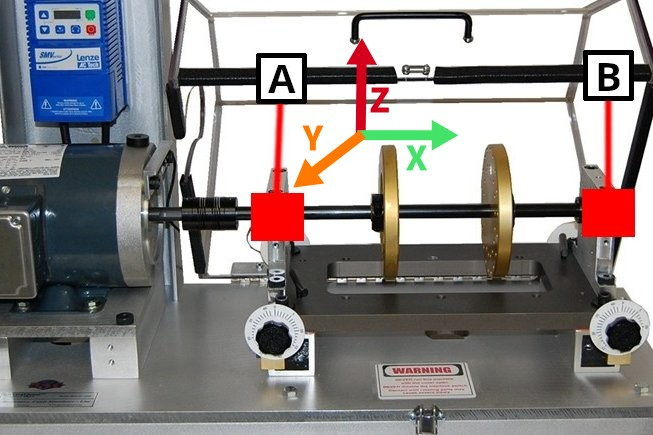
\includegraphics[width=\textwidth]{fig/sensor/mafaulda-simulator.jpg}
         \caption{MaFaulDa}
         \label{fig:mafaulda-simulator}
     \end{subfigure}
     \hfill
     \begin{subfigure}[b]{0.24\textwidth}
         \centering
         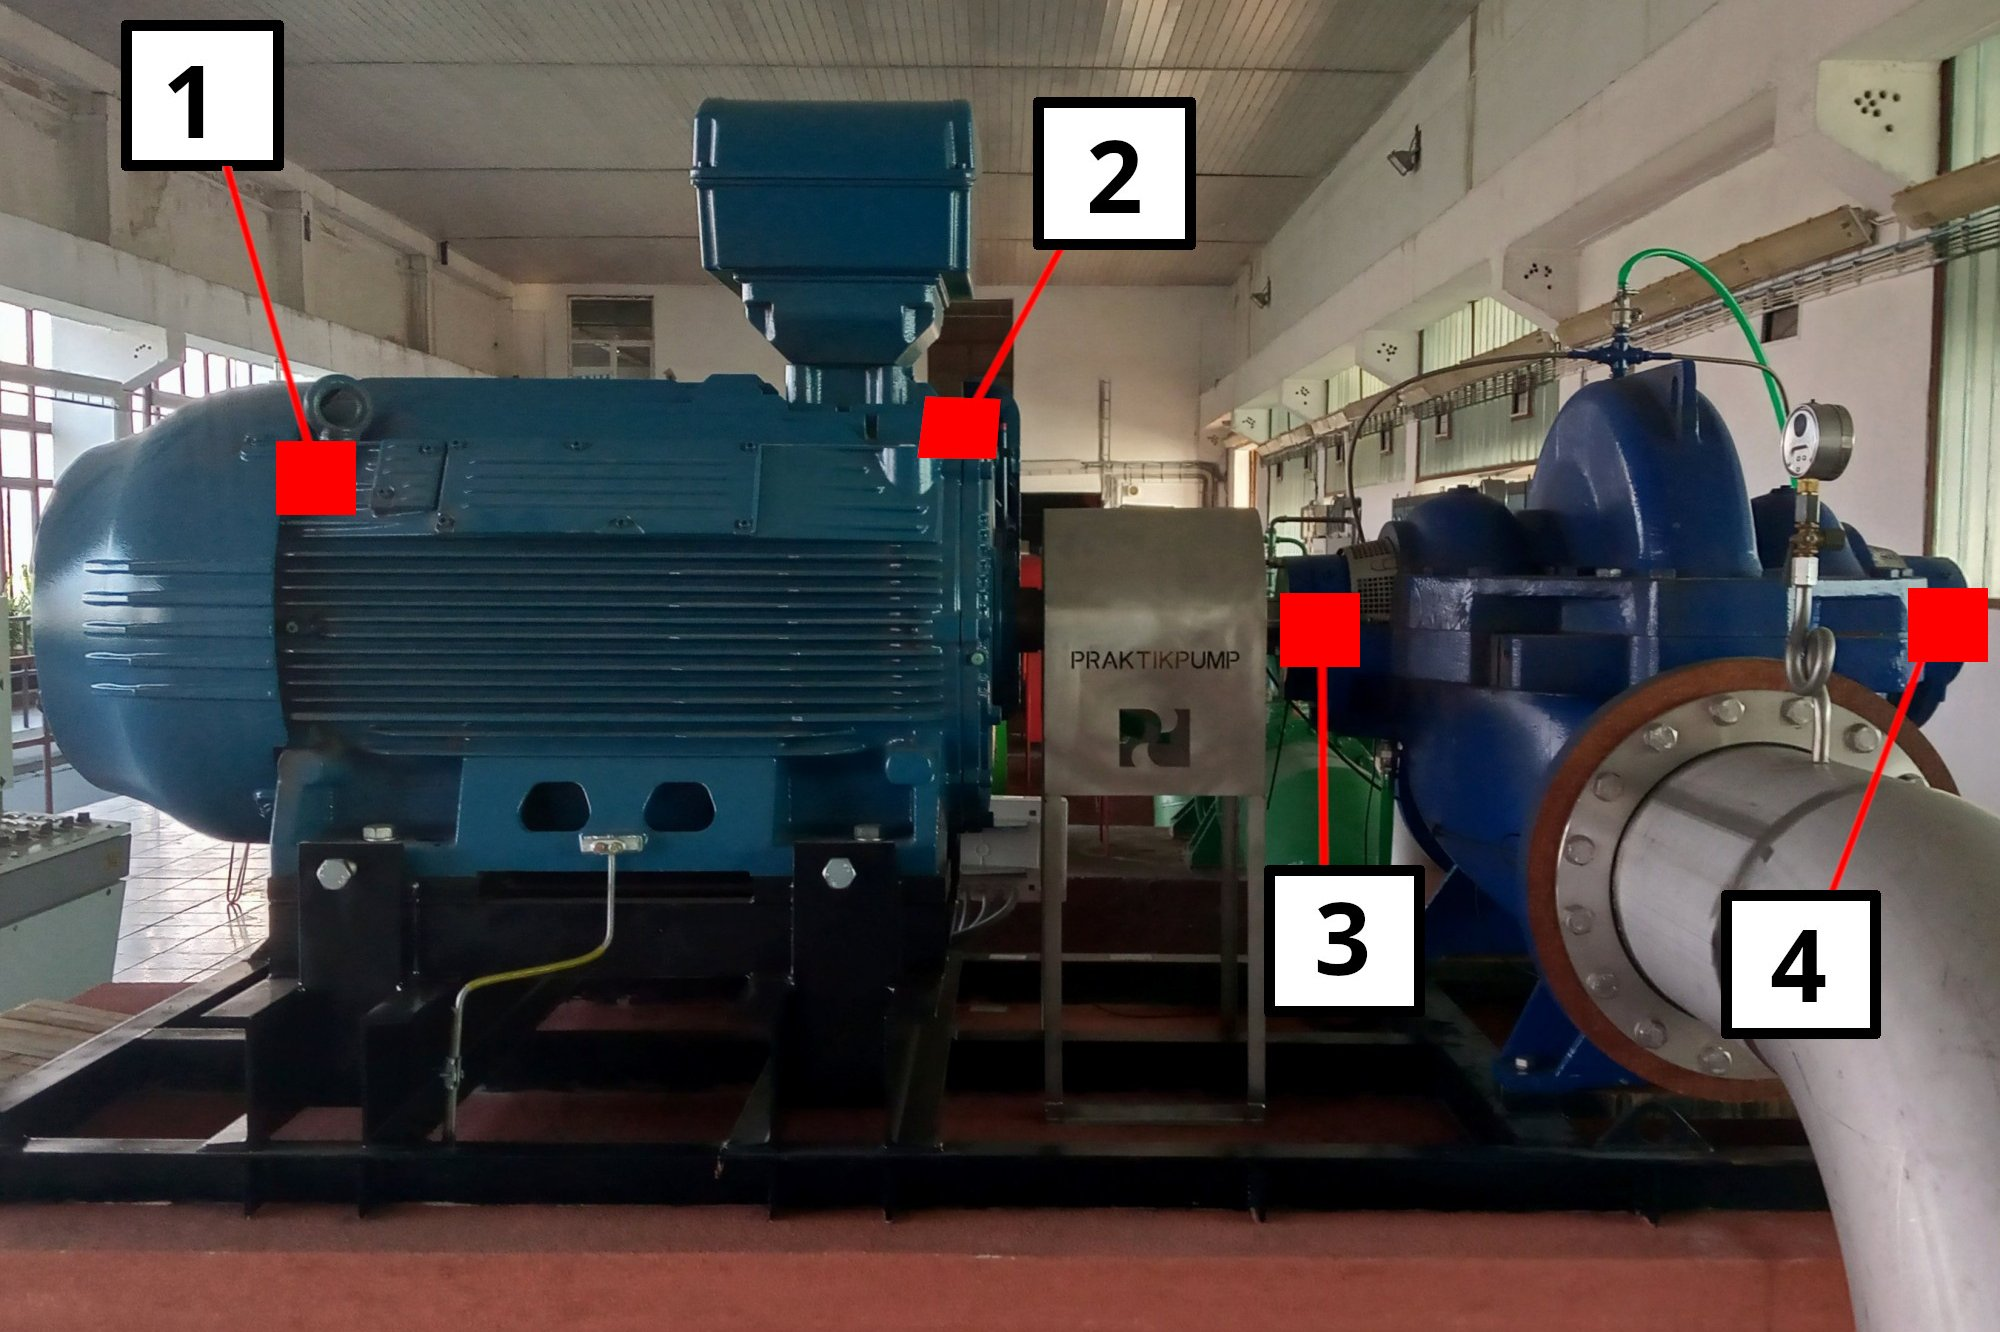
\includegraphics[width=\textwidth]{fig/sensor/ksb-pump.jpg}
         \caption{Water pump}
         \label{fig:water-pump}
     \end{subfigure}
     \hfill
     \begin{subfigure}[b]{0.24\textwidth}
         \centering
         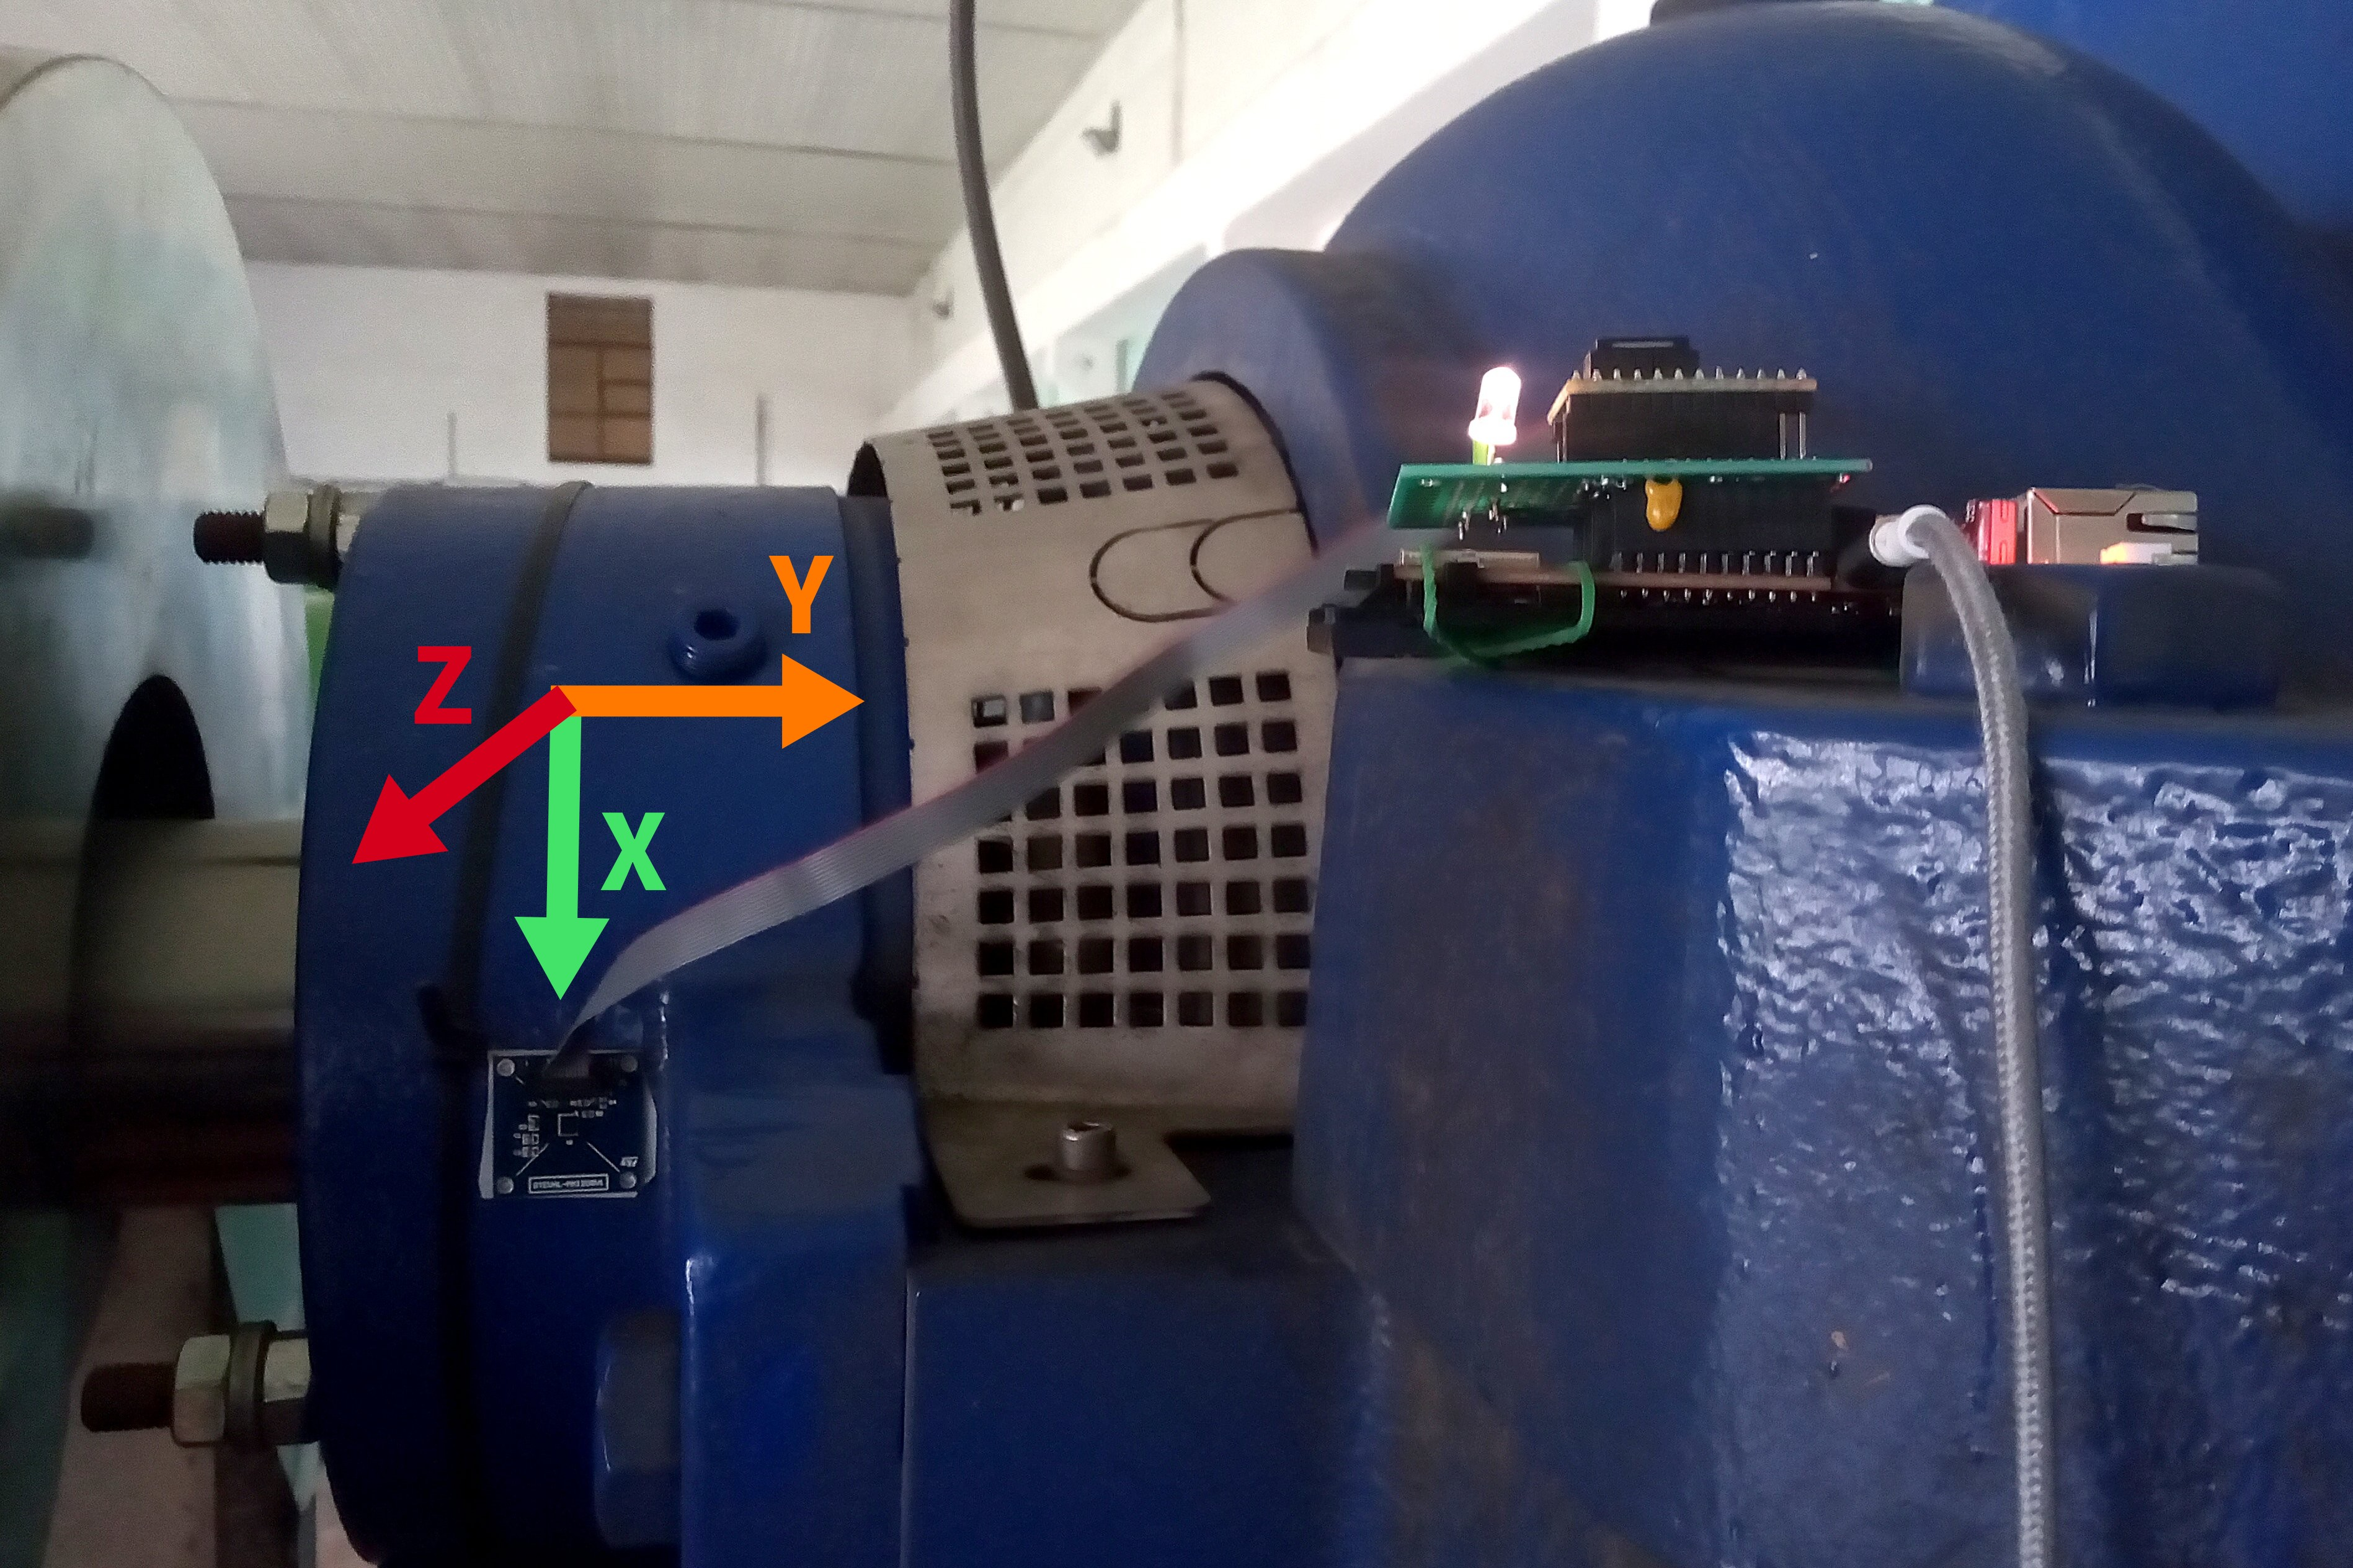
\includegraphics[width=\textwidth]{fig/sensor/sensor.jpg}
         \caption{Accelerometer}
         \label{fig:steval-sensor}
     \end{subfigure}
     \hfill
     \begin{subfigure}[b]{0.24\textwidth}
         \centering
         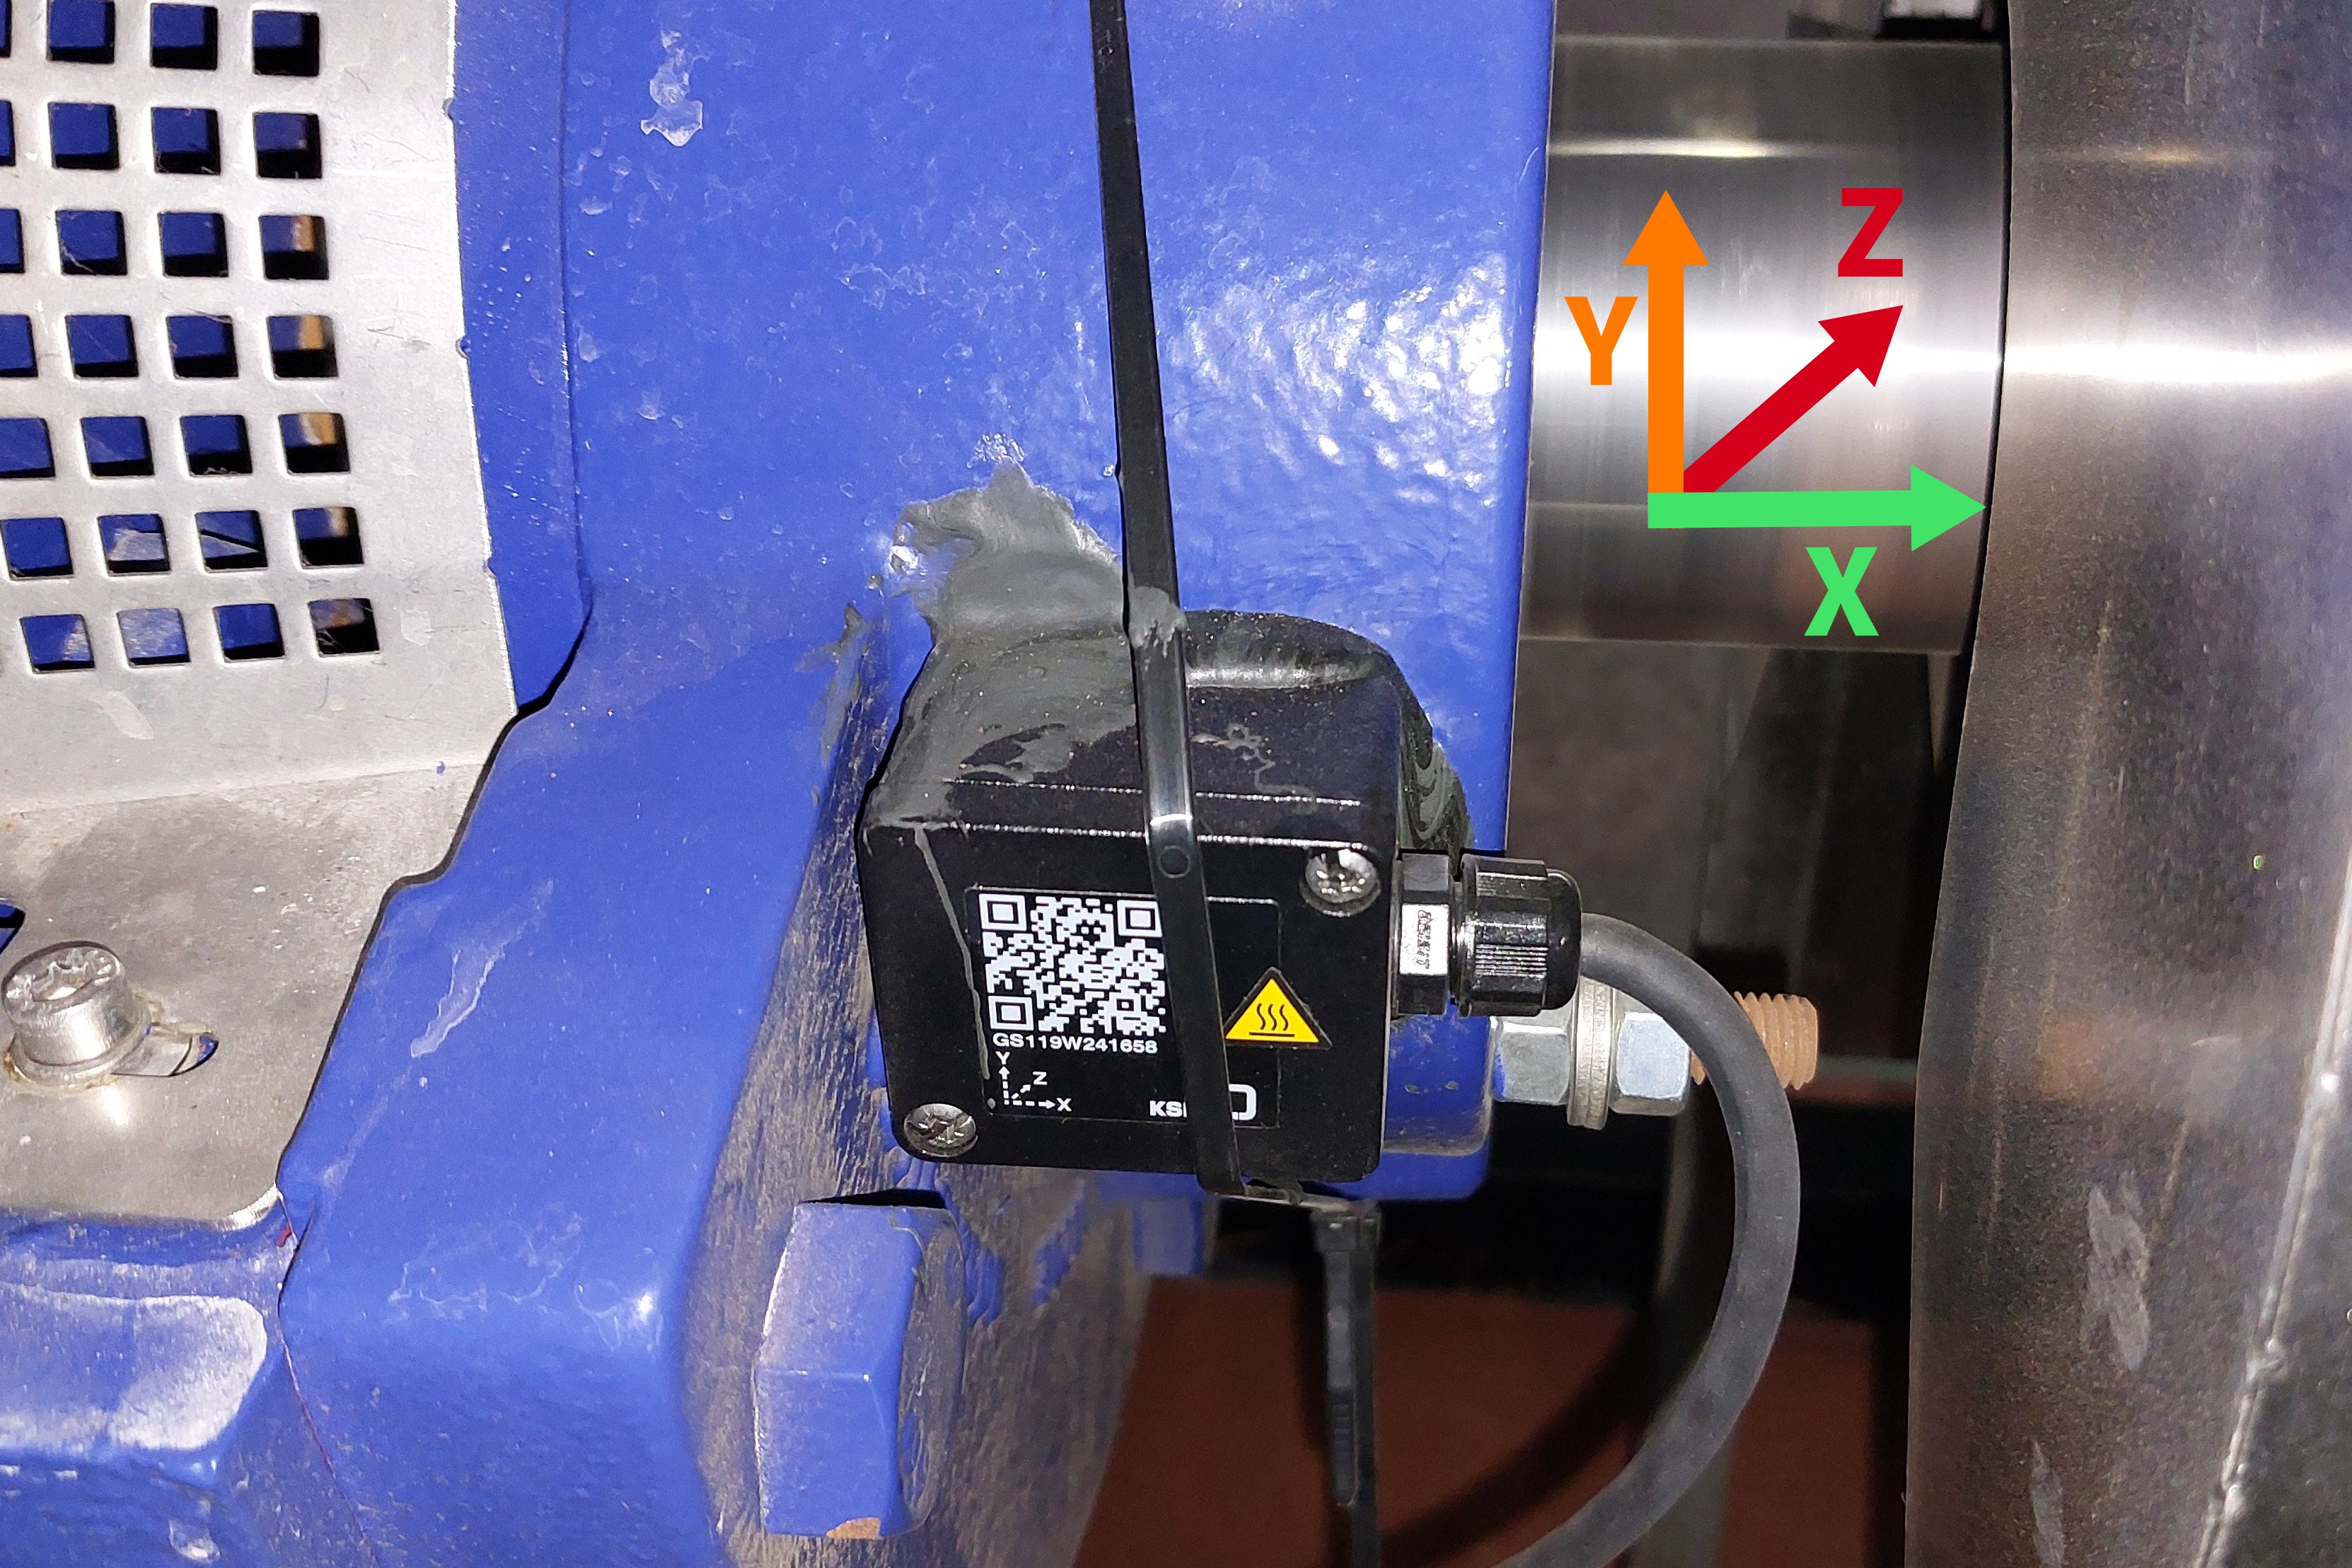
\includegraphics[width=\textwidth]{fig/sensor/ksb-cloud.jpg}
         \caption{KSB sensor}
         \label{fig:ksb-cloud-sensor}
     \end{subfigure}
     \caption{Measurement positions and accelerometer orientations}
\end{figure}

Data preprocessing of MaFaulDa is necessary to create feature sets in TD and FD. This process of several phases.
\begin{enumerate}
\item \textbf{Signal filtering}: Subtraction of overall mean removes DC component. IIR Butterworth low pass filter of 5th order attenuates frequencies above above 10 kHz.
\item \textbf{Feature extraction}: Machine behavior in one time series is time-invariant therefore each feature is calculated out of whole duration. Frequency domain features are produced using Welch's method for power spectrums from FFT with $2^{15}$ long Hann windows and 50\% overlap  (bin resolution of 1.53~Hz). The resulting features belong to domains making up respective feature sets:
\begin{enumerate}
\item \textbf{10 time domain features} (TD): peak-to-peak amplitude, zero-crossing rate, root mean square, skewness, kurtosis, shape factor, crest factor, impulse factor, clearance factor, average amplitude change,
\item \textbf{11 frequency domain features} (FD): spectral centroid, standard deviation, skewness, kurtosis, roll on frequency of 5\% total energy, roll off frequency of 85\% total energy, spectral flux as a average correlation of separate windows, noisiness as a signal to noise ratio, spectral negentropy~\cite{avoci_spectral_2020}, energy, entropy.
\end{enumerate}
\item \textbf{Labeling}: Three target variables are constructed out of inner bearing, both bearings, and high severity defects on both bearings. Predicted variable has 6 classes: normal, misalignment (merged vertical and horizontal), imbalance, outer race fault, ball fault, cage fault. In high severity scenario, the normal class is assigned to observations where weight or shaft shift applied is in half below 60\% of all configuations for that fault.
\item \textbf{Class balancing}: Random oversampling strategy is used on all classes except the majority one.
\end{enumerate}

Vibrations from pumps in municipal pumping station for drinking water in Podunajské Biskupice reveal practical challenges for deployment of machine learning models in the industry. Two pumps (P1, P2) of the same type KSB Omega 300-560 and two electric motors WEG W50 (M1, M2) were designated for measurements. Both machines have power 400~kW (ISO 20186 class~\rom{3}) and main shaft rotates at 1493~RPM. For purposes of expert labeling, the bearing designations at numbered places are: 6319-C3 (1), 6324-C3 (2), 6317-2Z (3 \& 4). 

Sensor were placed above bearings in numbered positions according to ISO 13373 (Fig.~\ref{fig:water-pump}) with axis orientation depicted in Fig.~\ref{fig:steval-sensor}. Each pump is equipped with KSB cloud monitoring at place (3) (Fig.~\ref{fig:ksb-cloud-sensor}) from which rms velocity in mm/s is available for year in hourly intervals. 

Our accelerometer ST IIS3DWB mounted to machine unig thin double sided tape has wideband 5 kHz linear response is sampled at 26.87~kHz. Microcontroller ESP32-POE-ISO stored triaxial 60 second long recordings onto SD card. In total 48 time series were gathered, 6 in each place. These are furter split to 5 second interval for 576 data points overall.

The signal preprocessing is similiar which exceptions that low-pass filter is left out and FFT window size is set to $2^{14}$ (bin resolution of 1.64~Hz). Fault labels are missing therefore we analyse rotational speeds and defect bearing frequencies in the frequency spectrum. As an alternative, the observations are labeled based on source machinery to 4 classes: M1, M2, P1, P2; based on sensor position to 8 classes: M1-1, M1-2, P1-3, P1-4, etc. Another classfier is made solely with P1-3 and P2-3 placements.
Classification is done for features in main axis of motion (z) and euclidian norm of same features in all directions.


\section{Results}
\begin{figure}
     \begin{subfigure}[b]{0.3\textwidth}
         \centering
         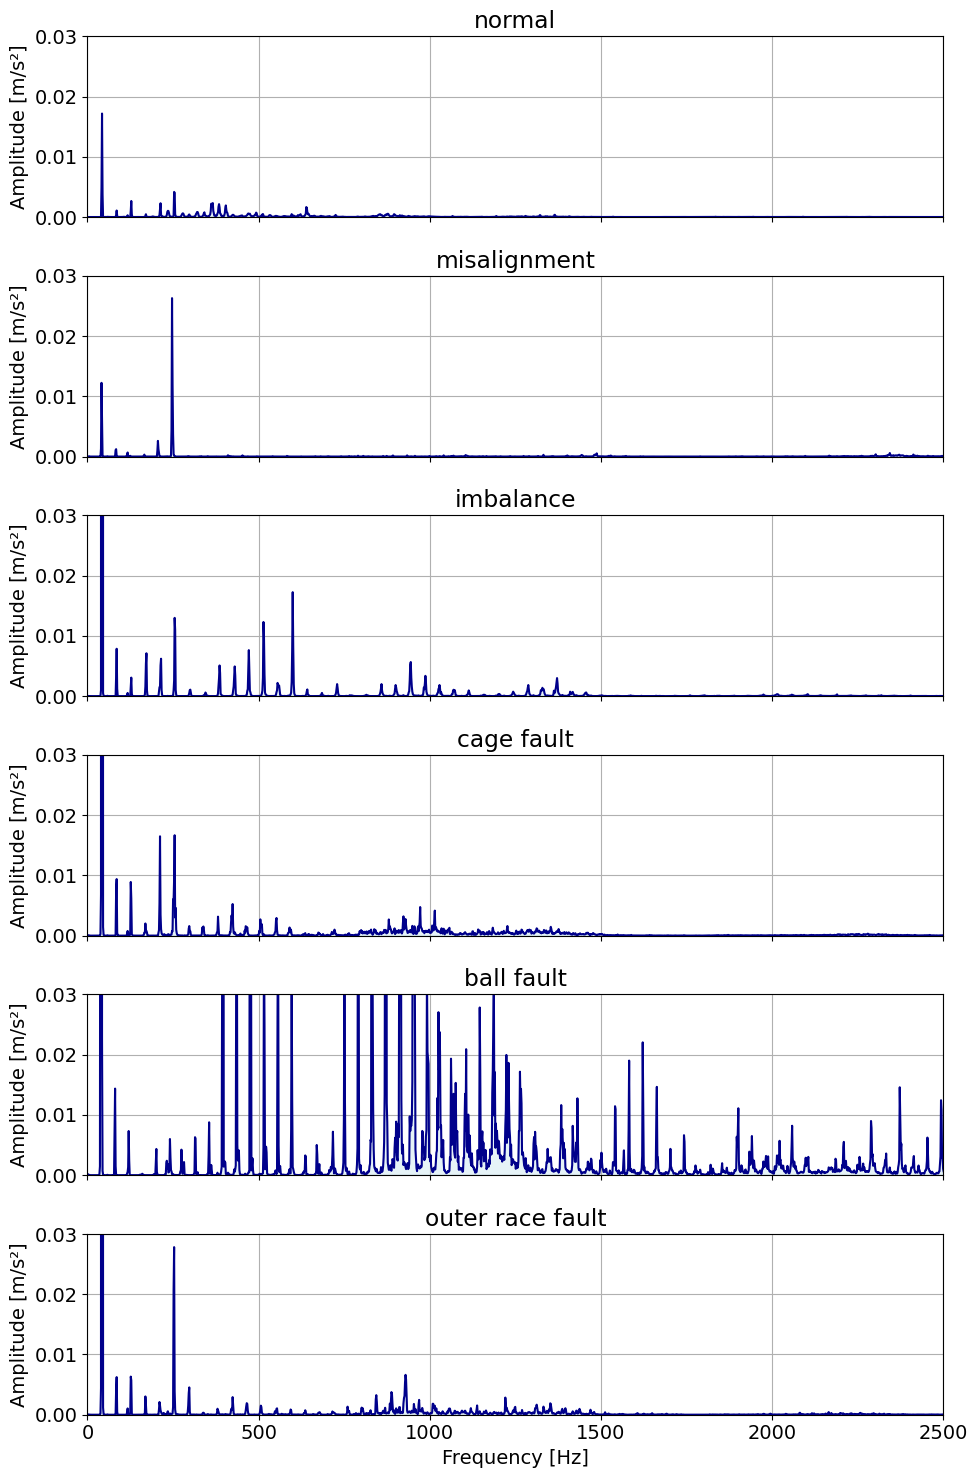
\includegraphics[width=\textwidth]{fig/spectrum/mafaulda-wideband.png}
         \caption{MaFaulda}
         \label{fig:mafaulda-wideband}
     \end{subfigure}
     \hfill
     \begin{subfigure}[b]{0.3\textwidth}
         \centering
         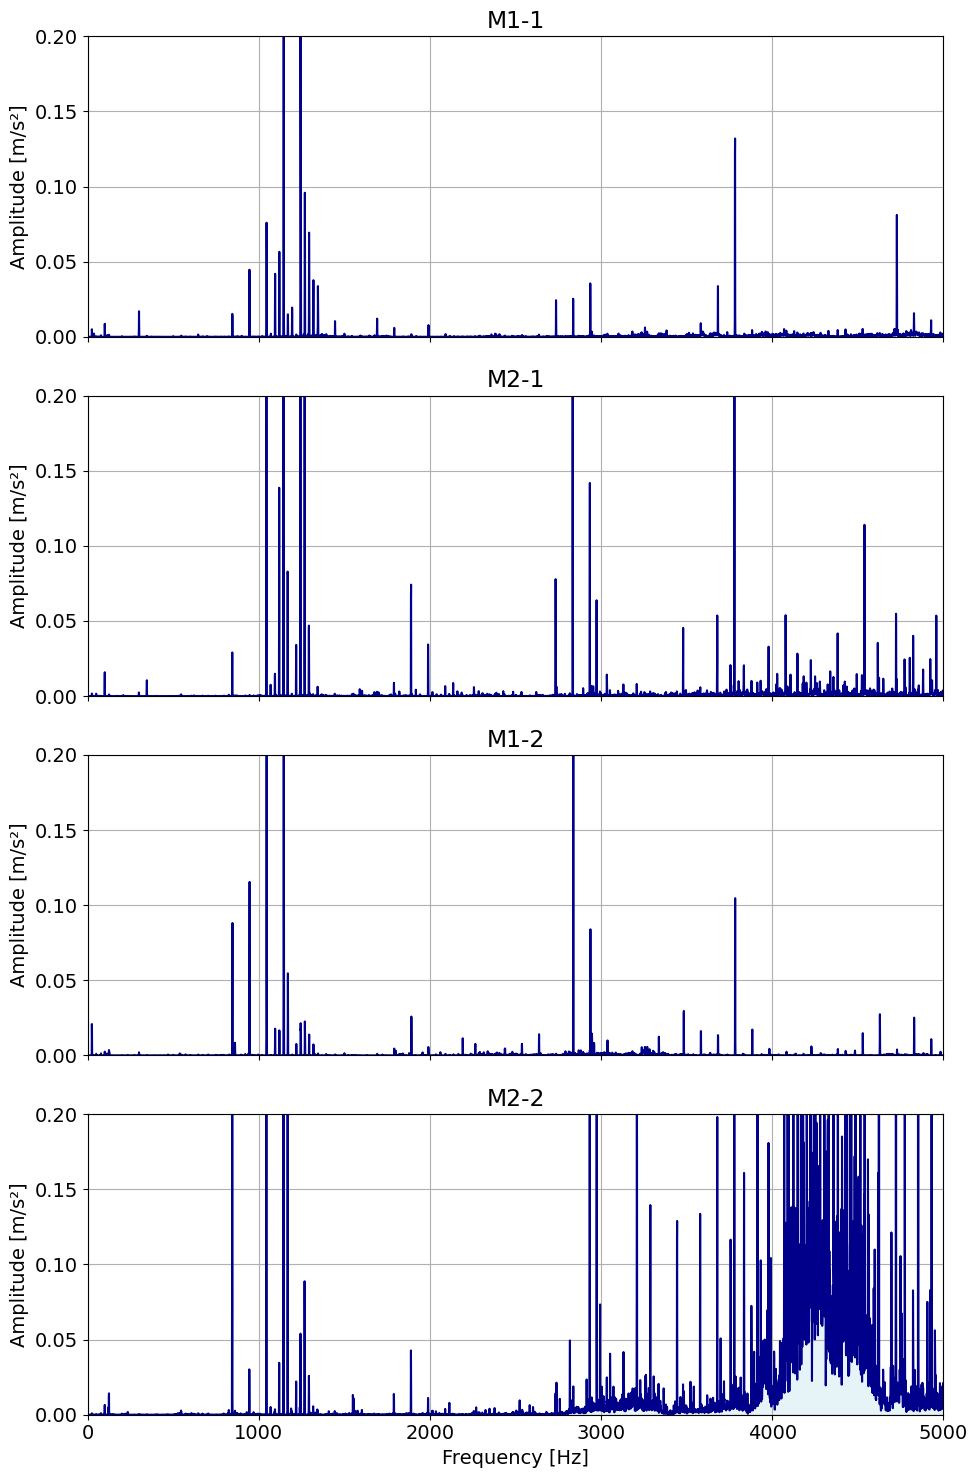
\includegraphics[width=\textwidth]{fig/spectrum/motor-wideband.png}
         \caption{Motors}
         \label{fig:motor-wideband}
     \end{subfigure}
     \hfill
     \begin{subfigure}[b]{0.3\textwidth}
         \centering
         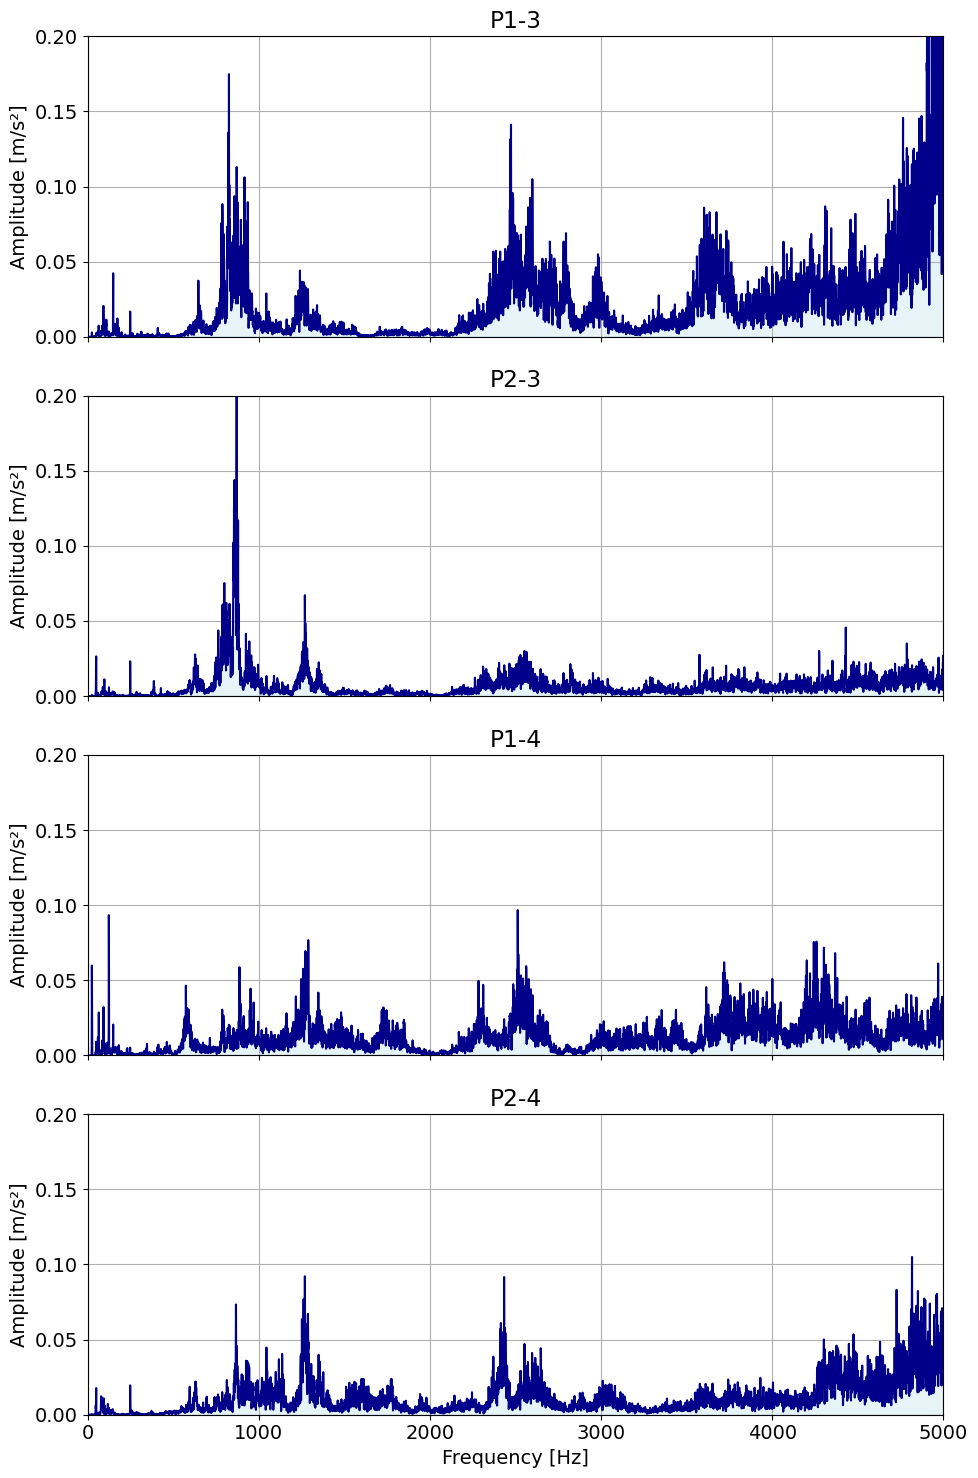
\includegraphics[width=\textwidth]{fig/spectrum/pump-wideband.png}
         \caption{Pumps}
         \label{fig:motor-wideband}
     \end{subfigure}
     \caption{Wideband power spectrum}
\end{figure}

\begin{figure}
     \begin{subfigure}[b]{0.3\textwidth}
         \centering
         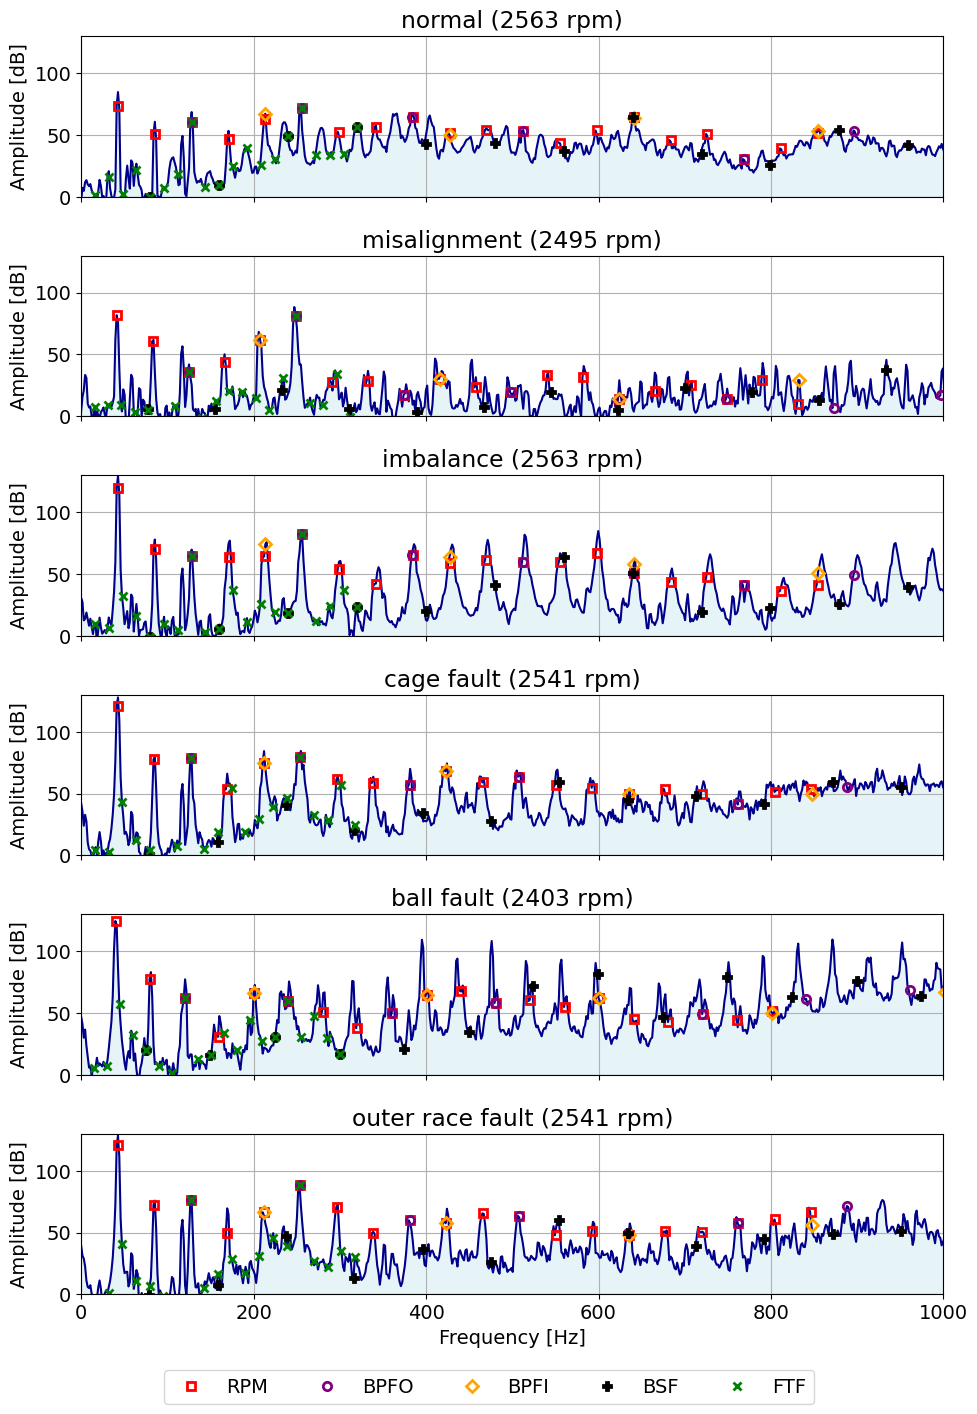
\includegraphics[width=\textwidth]{fig/spectrum/mafaulda-fault.png}
         \caption{MaFaulda}
         \label{fig:mafaulda-fault}
     \end{subfigure}
     \hfill
     \begin{subfigure}[b]{0.3\textwidth}
         \centering
         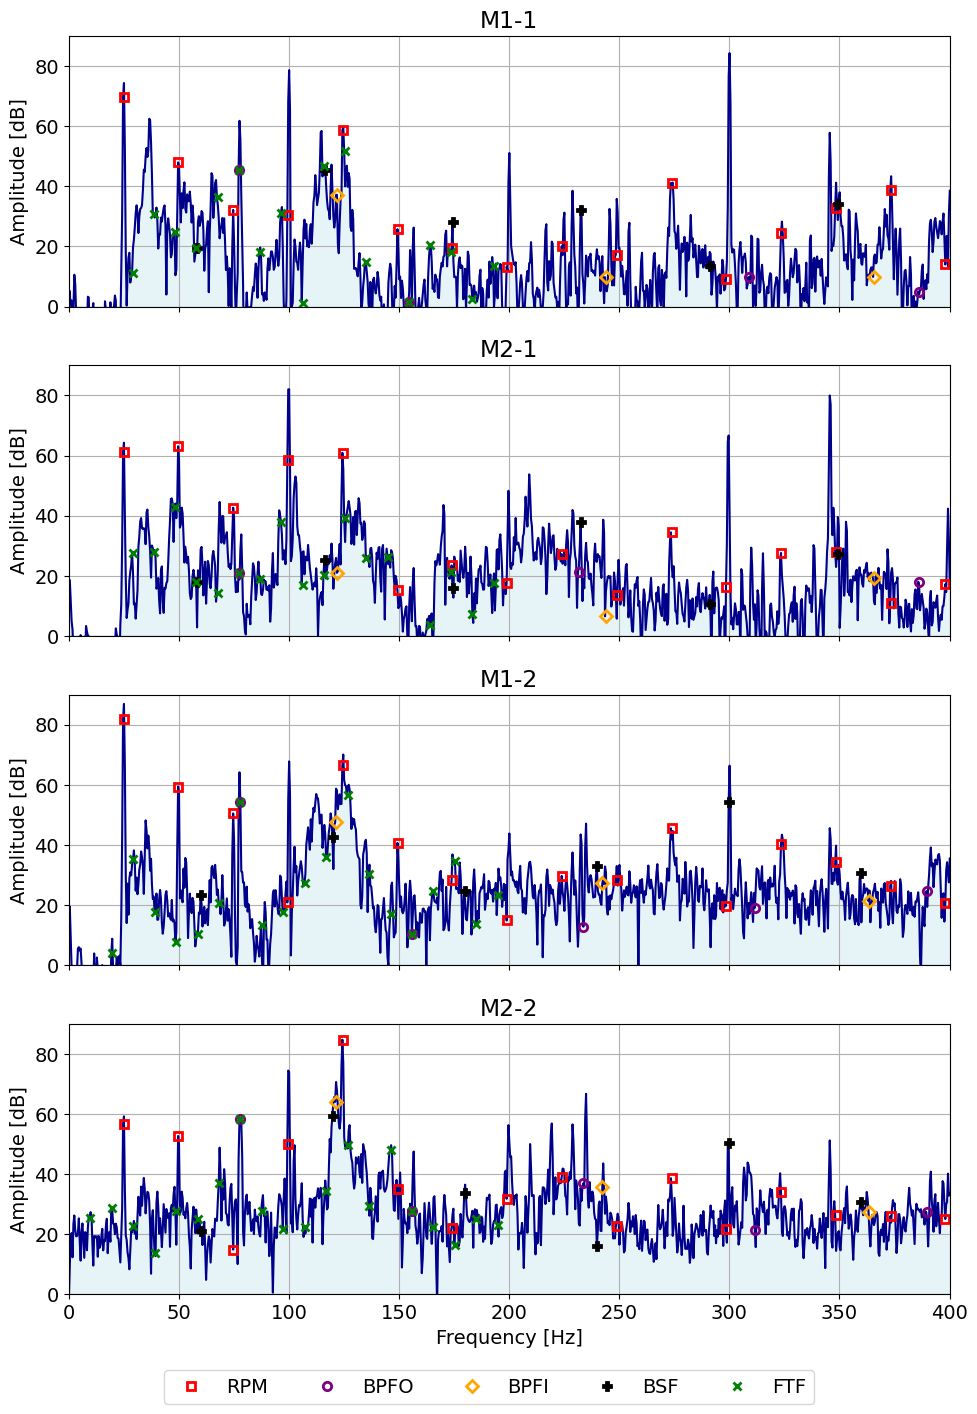
\includegraphics[width=\textwidth]{fig/spectrum/motor-fault.png}
         \caption{Motors}
         \label{fig:motor-fault}
     \end{subfigure}
     \hfill
     \begin{subfigure}[b]{0.3\textwidth}
         \centering
         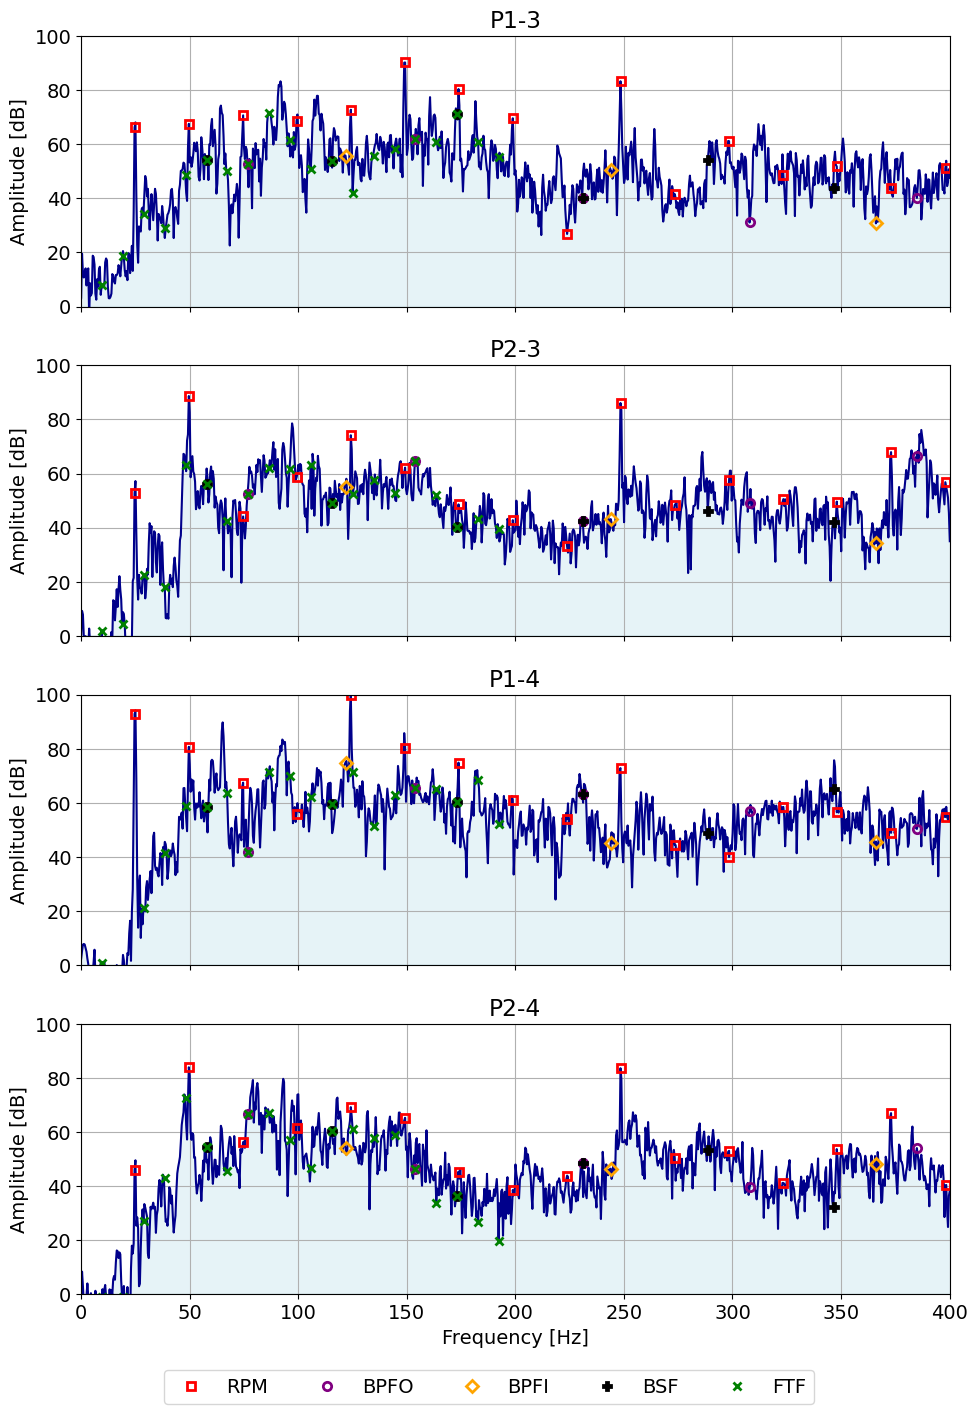
\includegraphics[width=\textwidth]{fig/spectrum/pump-fault.png}
         \caption{Pumps}
         \label{fig:pump-fault}
     \end{subfigure}
     \caption{Shaft and bearing defect frequencies}
\end{figure}


\begin{table}
\centering
\caption{Numbers of observations by label in MaFaulDa}\label{tab:mafaulda-observation-counts}
\begin{tabular}{|l|r|r|r|}
\hline
\textbf{Label} &  \textbf{Bearing A} & \textbf{Both bearings} & \textbf{High severity} \\
\hline
normal            &  49  &  49  &  1125 \\
misalignment      & 498  &  498 & 198 \\
imbalance         & 333  &  333 & 139 \\
cage fault        & 188  &  376 & 181 \\
ball fault        & 186  &  323 & 132 \\
outer race fault  & 184  &  372 & 176 \\
\hline
$\Sigma$ & 1438  & 1951 & 1951 \\
\hline
\end{tabular}
\end{table}

\begin{figure}
     \begin{subfigure}[b]{0.48\textwidth}
         \centering
         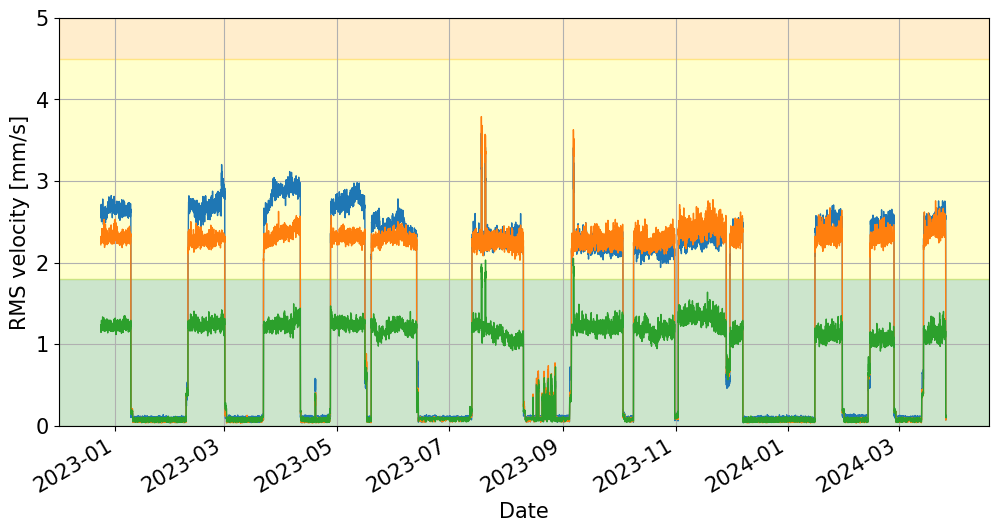
\includegraphics[width=\textwidth]{fig/ksb-cloud/P1-rms-vibration.png}
         \caption{P1-3}
         \label{fig:P1-ksb-rms}
     \end{subfigure}
     \hfill
     \begin{subfigure}[b]{0.48\textwidth}
         \centering
         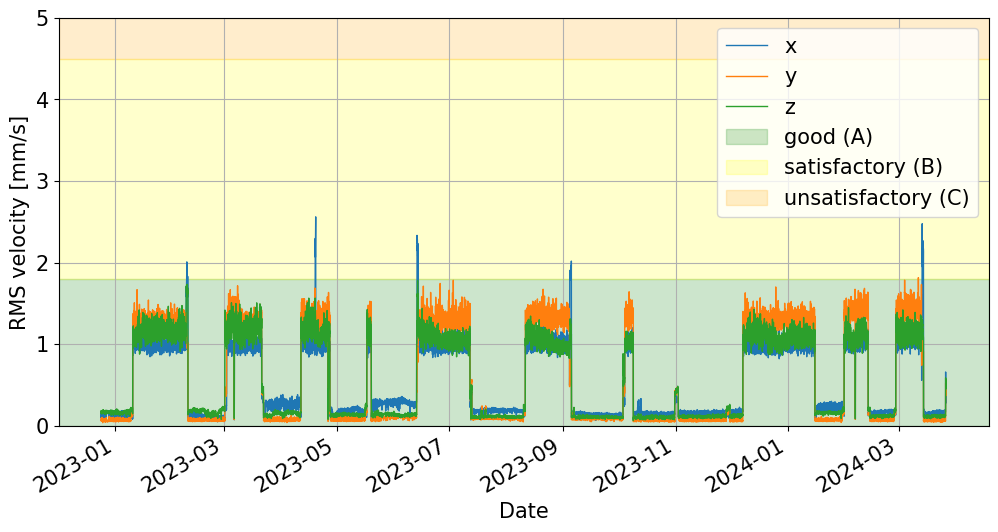
\includegraphics[width=\textwidth]{fig/ksb-cloud/P2-rms-vibration.png}
         \caption{P2-3}
         \label{fig:P2-ksb-rms}
     \end{subfigure}
     \caption{RMS vibrations of pumps and ISO severity levels}
\end{figure}


% Identical plots for one axis and multiple axis
\begin{figure}
     \begin{subfigure}[b]{0.32\textwidth}
         \centering
         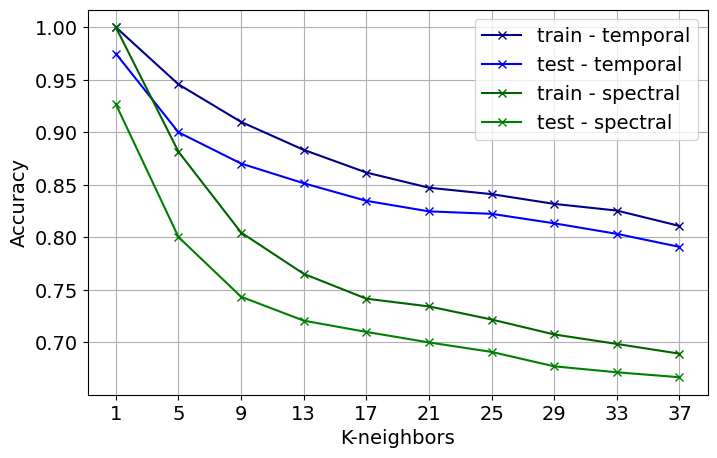
\includegraphics[width=\textwidth]{fig/all-features-mafaulda/all-axis-a-bearing.png}
         \caption{Bearing A}
     \end{subfigure}
     \hfill
     \begin{subfigure}[b]{0.32\textwidth}
         \centering
         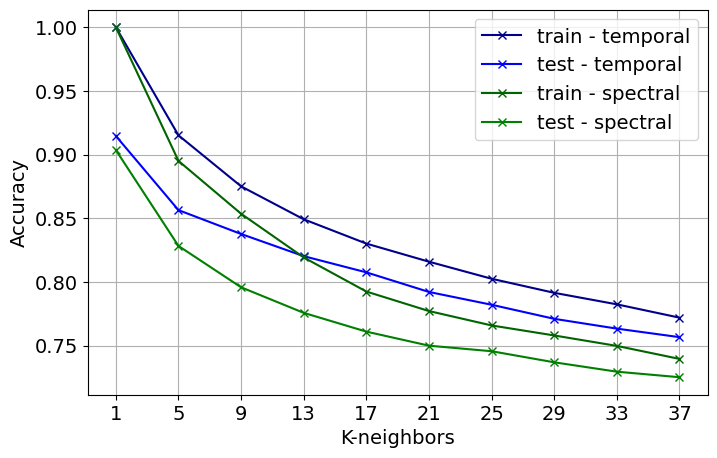
\includegraphics[width=\textwidth]{fig/all-features-mafaulda/all-axis-all-bearings.png}
         \caption{Both bearings}
     \end{subfigure}
     \hfill
     \begin{subfigure}[b]{0.32\textwidth}
         \centering
         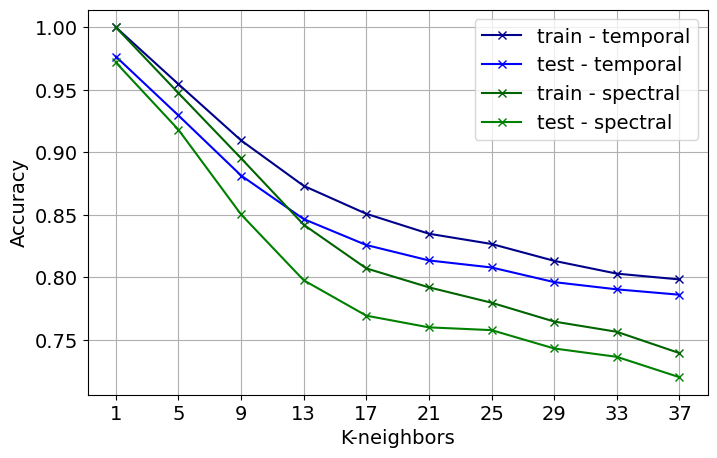
\includegraphics[width=\textwidth]{fig/all-features-mafaulda/all-axis-severity.png}
         \caption{High severity}
     \end{subfigure}
     \caption{Whole feature sets in TD and FD from MaFaulDa}
\end{figure}



\begin{figure}
     \begin{subfigure}[b]{0.32\textwidth}
         \centering
         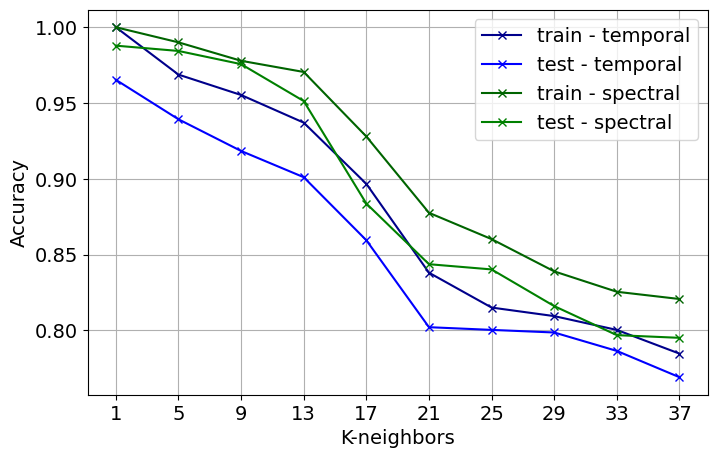
\includegraphics[width=\textwidth]{fig/all-features-pumps/machine.png}
         \caption{Machines}
     \end{subfigure}
     \hfill
     \begin{subfigure}[b]{0.32\textwidth}
         \centering
         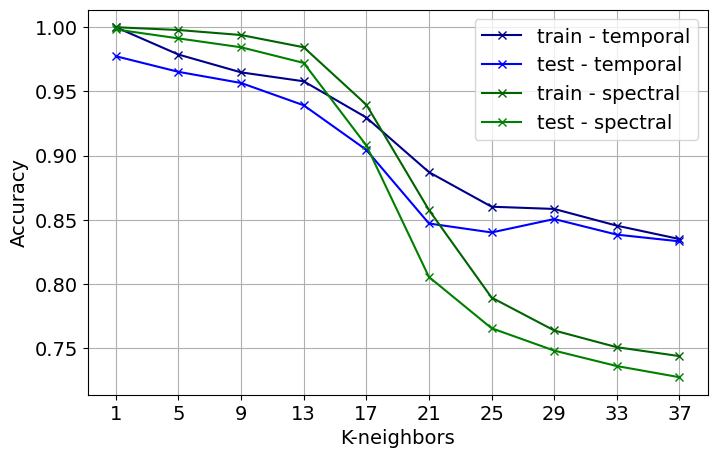
\includegraphics[width=\textwidth]{fig/all-features-pumps/position.png}
         \caption{Positions}
     \end{subfigure}
     \hfill
     \begin{subfigure}[b]{0.32\textwidth}
         \centering
         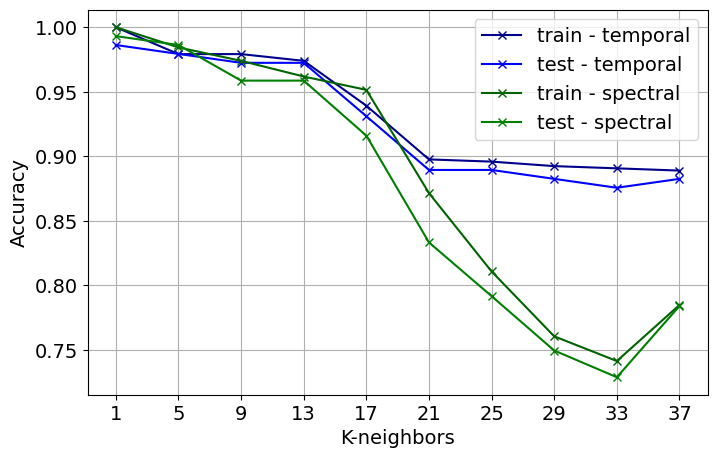
\includegraphics[width=\textwidth]{fig/all-features-pumps/binary.png}
         \caption{Pumps on position 3}
     \end{subfigure}
     \caption{Whole feature sets in TD and FD from water pumps}
\end{figure}


% All bearings
\begin{figure}
	\centering
     \begin{subfigure}[b]{0.45\textwidth}
         \centering
         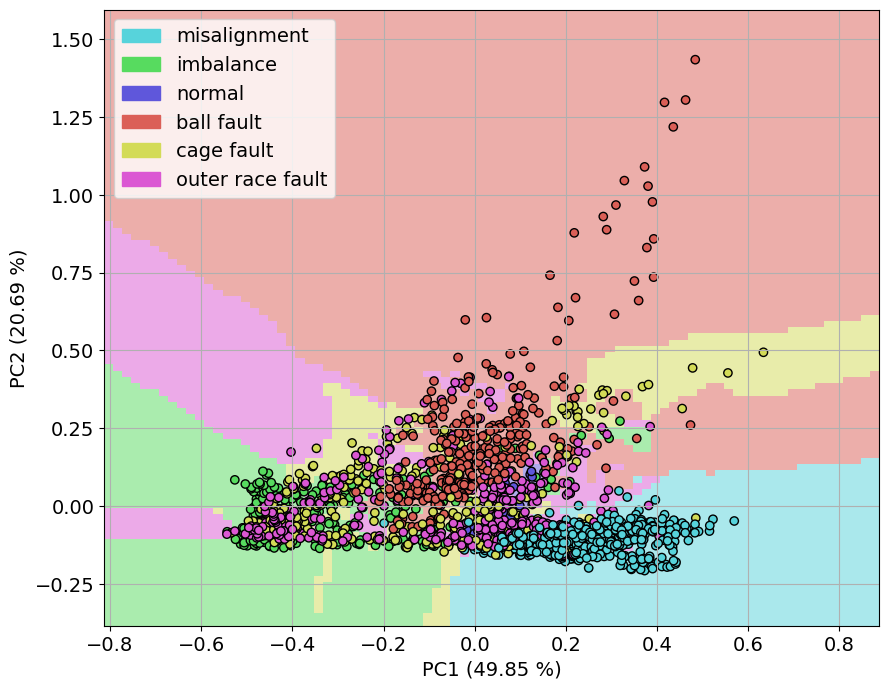
\includegraphics[width=\textwidth]{fig/scatter-mafaulda/td-all-bearings.png}
         \caption{Both bearings in TD}
     \end{subfigure}
     \hfill
     \begin{subfigure}[b]{0.45\textwidth}
         \centering
         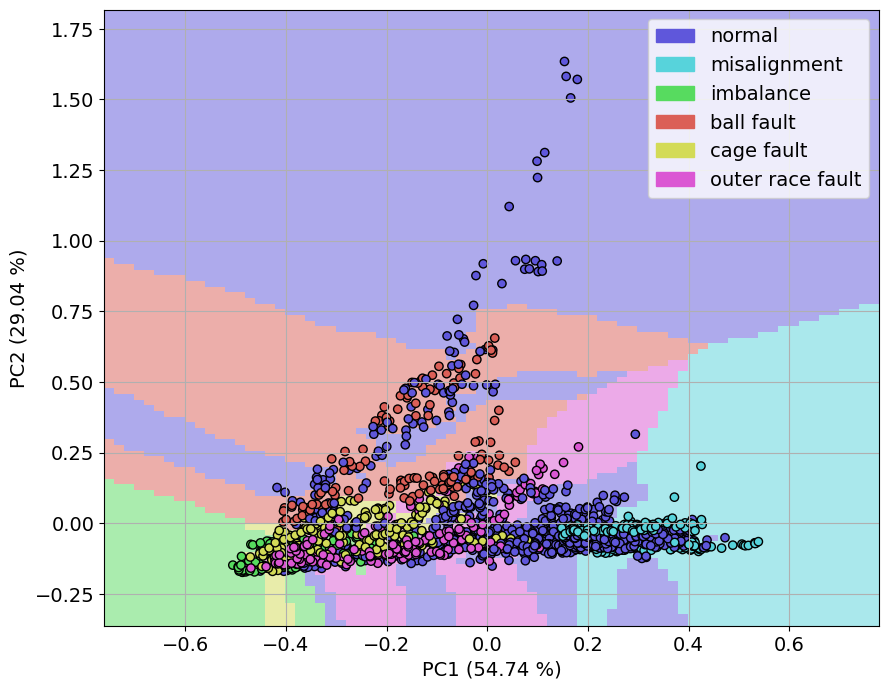
\includegraphics[width=\textwidth]{fig/scatter-mafaulda/td-severity.png}
         \caption{High severity in TD}
     \end{subfigure}
     \hfill
     \begin{subfigure}[b]{0.45\textwidth}
         \centering
         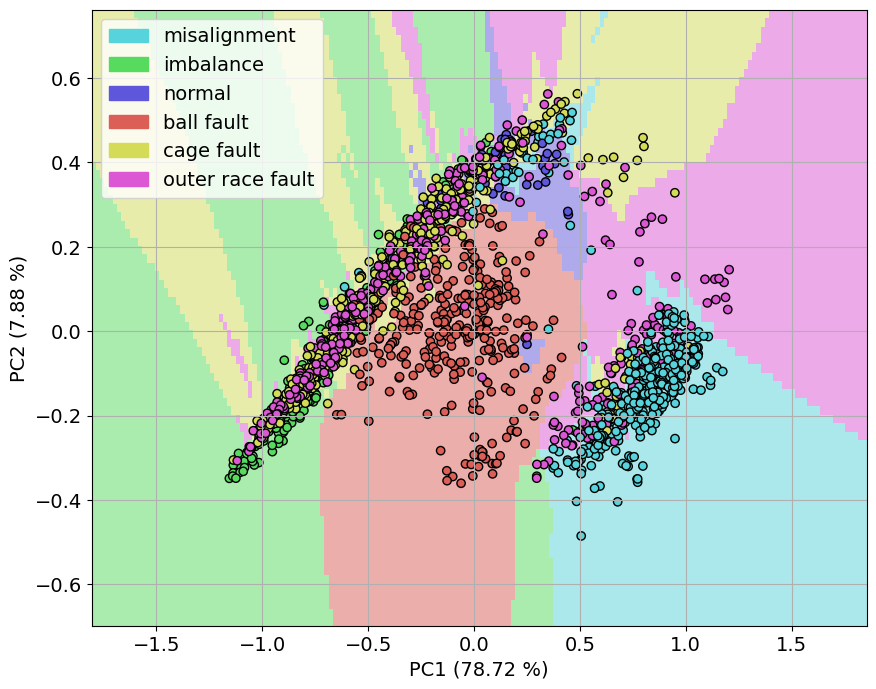
\includegraphics[width=\textwidth]{fig/scatter-mafaulda/fd-all-bearings.png}
         \caption{Both bearings in FD}
     \end{subfigure}
     \hfill
     \begin{subfigure}[b]{0.45\textwidth}
         \centering
         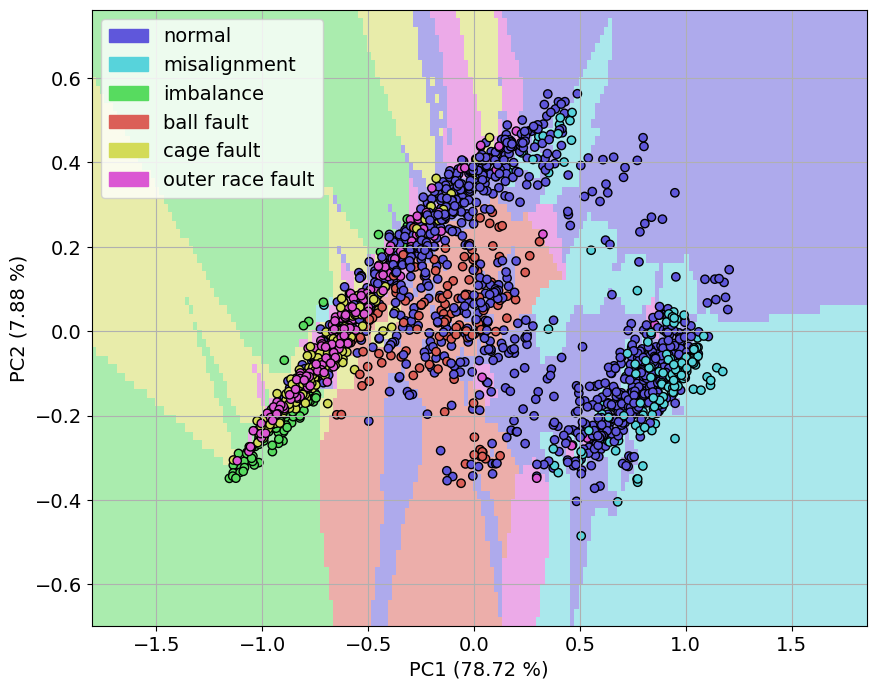
\includegraphics[width=\textwidth]{fig/scatter-mafaulda/fd-severity.png}
         \caption{High severity in TD}
     \end{subfigure}
     \caption{PCA scatter plots of MaFaulDa with k-NN decision boundaries (k = 5)}
\end{figure}


\begin{figure}
	\centering
     \begin{subfigure}[b]{0.45\textwidth}
         \centering
         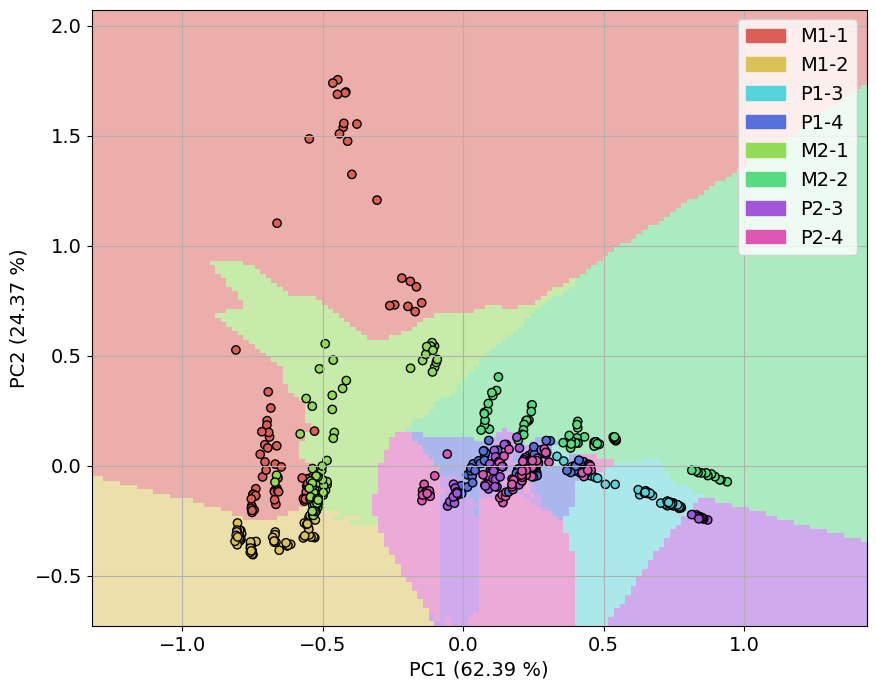
\includegraphics[width=\textwidth]{fig/scatter-pumps/position-td.png}
         \caption{Positions in TD}
     \end{subfigure}
     \hfill
     \begin{subfigure}[b]{0.45\textwidth}
         \centering
         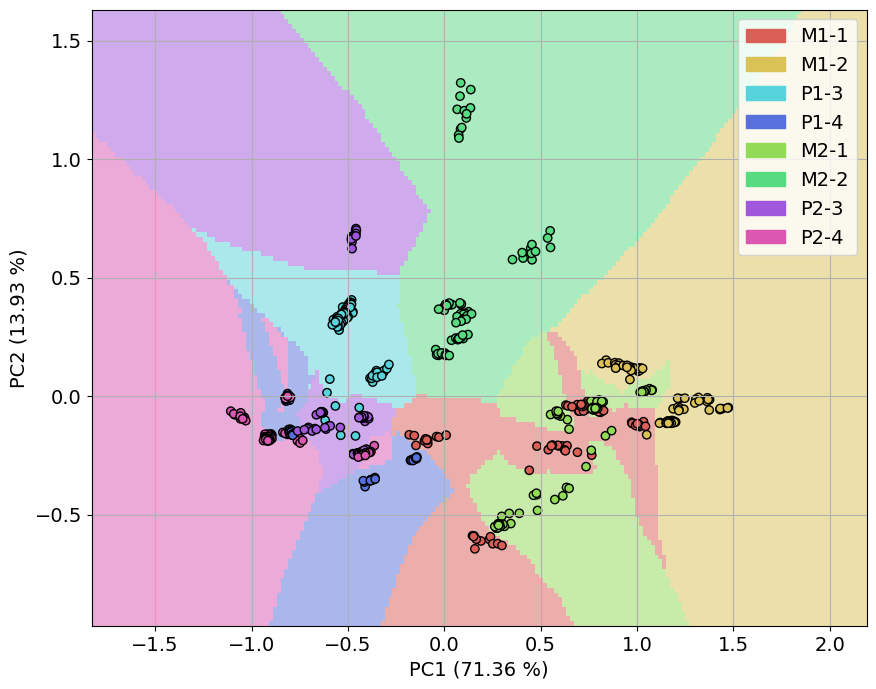
\includegraphics[width=\textwidth]{fig/scatter-pumps/position-fd.png}
         \caption{Positions in FD}
     \end{subfigure}
     \hfill
     \begin{subfigure}[b]{0.45\textwidth}
         \centering
         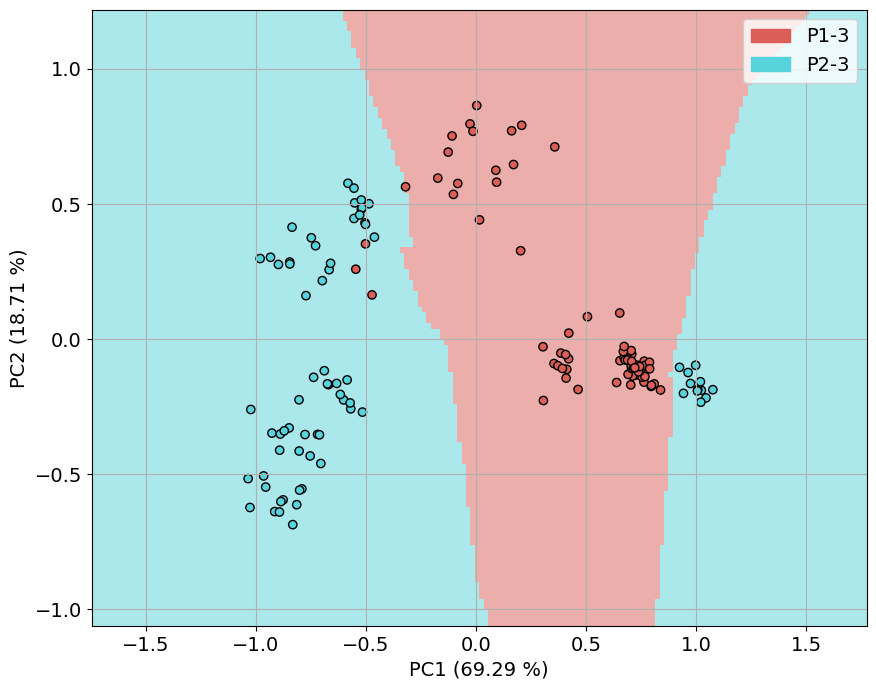
\includegraphics[width=\textwidth]{fig/scatter-pumps/binary-td.png}
         \caption{P1-3 and P2-3 in TD}
     \end{subfigure}
     \hfill
     \begin{subfigure}[b]{0.45\textwidth}
         \centering
         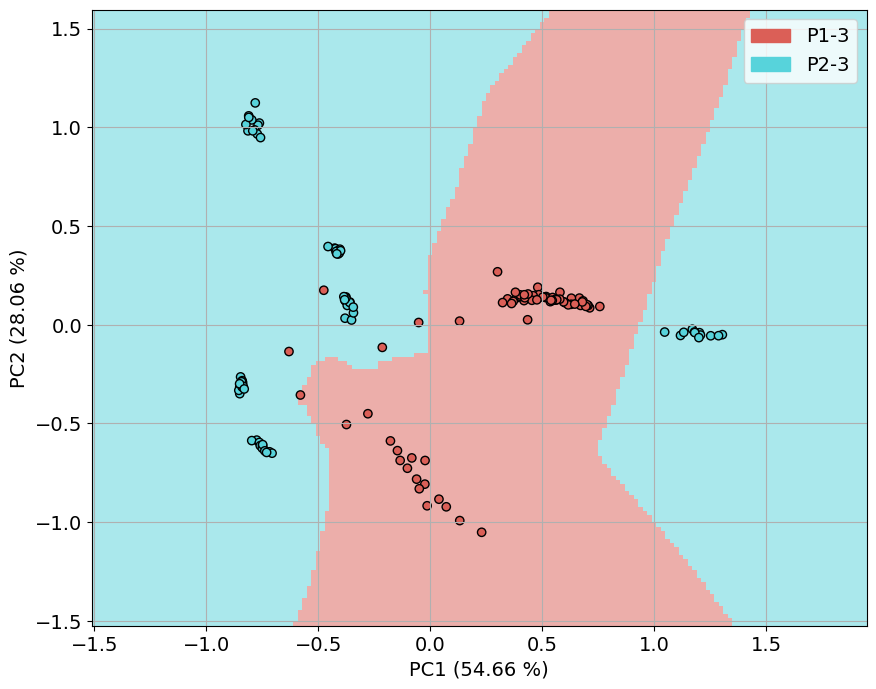
\includegraphics[width=\textwidth]{fig/scatter-pumps/binary-fd.png}
         \caption{P1-3 and P2-3 in FD}
     \end{subfigure}
     \caption{PCA scatter plots of water pumps with k-NN decision boundaries (k = 5)}
\end{figure}


% All axis
% by words relation to one axis, and one bearings
% Pumps - spectral is better
\begin{figure}
	\centering
     \begin{subfigure}[b]{0.45\textwidth}
         \centering
         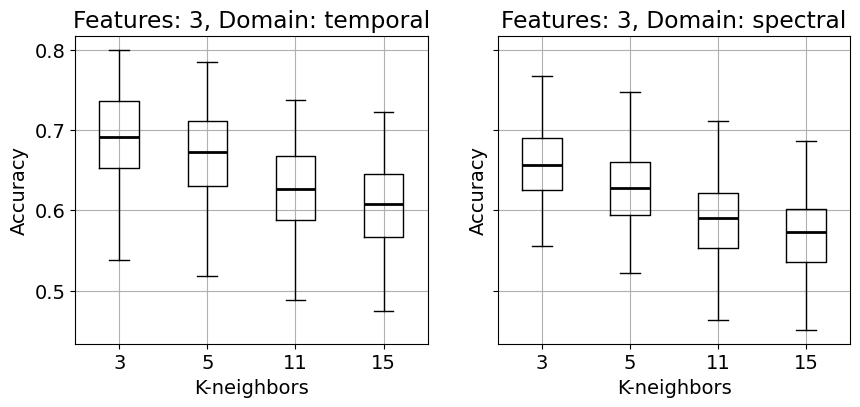
\includegraphics[width=\textwidth]{fig/combinations-mafaulda/all-axis-all-bearings-f3.png}
         \caption{Both bearings f=3}
     \end{subfigure}
     \hfill
     \begin{subfigure}[b]{0.45\textwidth}
         \centering
         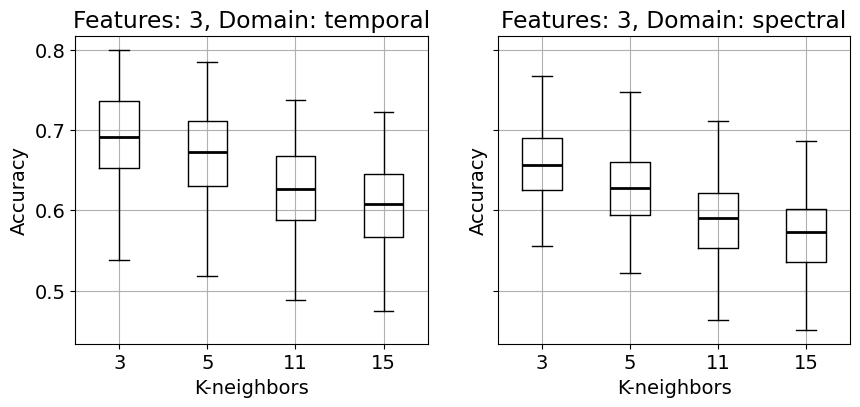
\includegraphics[width=\textwidth]{fig/combinations-mafaulda/all-axis-all-bearings-f3.png}
         \caption{Both bearings f=3}
     \end{subfigure}
     \hfill
     \begin{subfigure}[b]{0.45\textwidth}
         \centering
         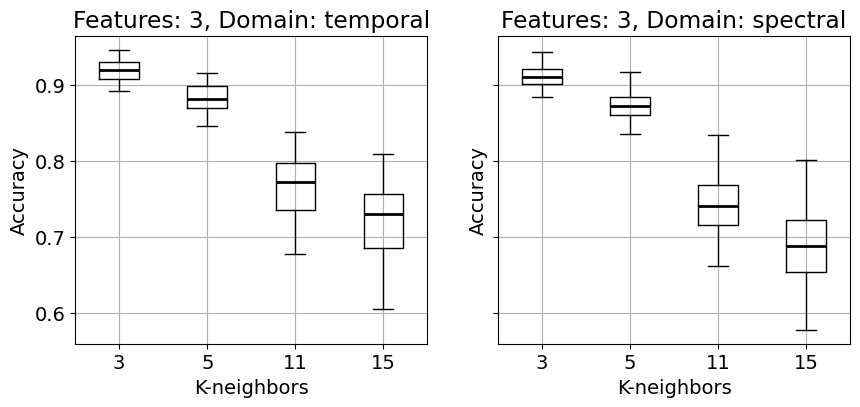
\includegraphics[width=\textwidth]{fig/combinations-mafaulda/all-axis-severity-f3.png}
         \caption{High severity k = 5}
     \end{subfigure}
     \hfill
     \begin{subfigure}[b]{0.45\textwidth}
         \centering
         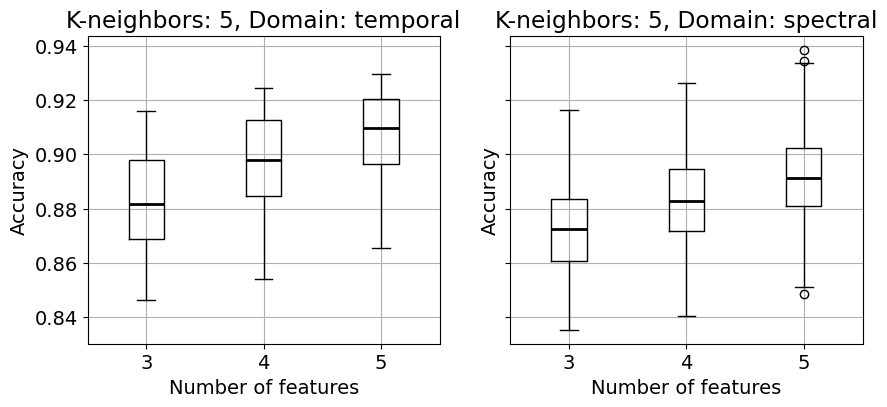
\includegraphics[width=\textwidth]{fig/combinations-mafaulda/all-axis-severity-k5.png}
         \caption{High severity k = 5}
     \end{subfigure}
     \caption{Test accuracies of all combinations of feature subsets}
\end{figure}

%TODO
% Table of accuracies for Maufaulda for rainbow bar plot (test set)

% Table for pumps

\section{Conclusions}


\section*{Acknowledgements}
We thank Lukáš Doubravský (R-DAS,~s.r.o.) for consultations on the methodology and assisting in sensor unit development. We appreciate domain experts in vibrodiagnostics prof.~Stanislav Žiaran and Dr.~Ondrej Chlebo (SjF~STU) for checking our approches. We also thank Peter Csóka and Peter Kmeťko (Bratislavská vodárenská spoločnosť,~a.s.) for enabling us access to water pumps.

\printbibliography



\end{document}
